\documentclass[11pt,aspectratio=169,xcolor=dvipsnames]{beamer}

% Impostazioni tema semplice e pulito
\usetheme{Boadilla}
\usecolortheme{default}
\setbeamertemplate{navigation symbols}{}

\setbeamercolor{title}{fg=PineGreen}
\setbeamercolor{frametitle}{fg=PineGreen}
\setbeamercolor{structure}{fg=PineGreen}
\setbeamerfont{frametitle}{series=\bfseries}

% Configurazione lingua e pacchetti
\usepackage[italian]{babel}
\usepackage[utf8]{inputenc}
\usepackage{graphicx}
\usepackage{amsmath}
\usepackage{booktabs}

% Dati per il frontespizio
\title{Progetto 1: Mini libreria di solutori iterativi per sistemi lineari SPD}
\subtitle{Metodi del Calcolo Scientifico}

\author{
    \begin{tabular}{rcl}
    Matias Bonoli & -- & matricola 912941 \\
    Ashley Chudory & -- & matricola 935003 \\
    Daniele Maccagnan & -- & matricola 945269
    \end{tabular}
}

\date{Anno accademico 2025/2026}

\begin{document}

\begin{frame}[plain]
    \titlepage
\end{frame}

\section{Introduzione}

\begin{frame}{Introduzione}
    \begin{itemize}
        \item Scopo del progetto è risolvere sistemi lineari con quattro metodi iterativi.
        \item La libreria si limita al caso di matrici simmetriche e definite positive.
        \item La parte che calcola la soluzione è scritta da zero usando le librerie standard solo per operazioni vettoriali elementari.
    \end{itemize}
\end{frame}

\section{I metodi e la libreria}

\begin{frame}{Criterio di arresto}
    \begin{itemize}
        \item L'iterazione si ferma quando il residuo diviso per $\|\mathbf{b}\|$ scende sotto la tolleranza, oppure se si supera il limite sul numero di iterazioni.
        \[ \frac{\|\mathbf{b} - A\mathbf{x}^{(k)}\|}{\|\mathbf{b}\|} < \text{tolleranza} \]
    \end{itemize}
\end{frame}

\begin{frame}{Splitting}
    \begin{itemize}
        \item I metodi stazionari si basano su uno splitting della matrice $A = P - N$, dove $P$ e $N$ non dipendono dall'iterazione.
        \item L'idea è scegliere $P$ in modo che sia facile da risolvere, ottenendo la formula iterativa:
        \[ \mathbf{x}^{(k+1)} = \mathbf{x}^{(k)} + P^{-1}\mathbf{r}^{(k)} \]
    \end{itemize}
\end{frame}

\begin{frame}{Metodo di Jacobi}
    \begin{itemize}
        \item Si prende come $P=D$ la diagonale di $A$ e come $N$ il resto con segno opposto.
        \[ \mathbf{x}^{(k+1)} = \mathbf{x}^{(k)} + D^{-1}\mathbf{r}^{(k)} \]
        \item Dato che $D$ è diagonale, la sua inversa è immediata e l'aggiornamento usa i valori dell'iterazione precedente.
        \item L'aggiornamento si fa con una operazione vettoriale, senza lenti cicli \texttt{for} di Python.
        \item Una iterazione costa quindi un prodotto matrice--vettore più operazioni vettoriali di ordine $O(n)$.
    \end{itemize}
\end{frame}

\begin{frame}{Metodo di Gauss-Seidel}
    \begin{itemize}
        \item Si prende come $P=L$ la parte triangolare inferiore di $A$, diagonale compresa.
        \[ \mathbf{x}^{(k+1)} = \mathbf{x}^{(k)} + L^{-1}\mathbf{r}^{(k)} \]
        \item La differenza rispetto a Jacobi è che si usano subito i valori già aggiornati in questa stessa iterazione.
        \item Non serve mai invertire la matrice: il sistema si risolve per sostituzione in avanti, che è sequenziale e non vettorizzabile.
        \item L'uso immediato dei valori aggiornati di solito fa convergere in meno iterazioni di Jacobi.
    \end{itemize}
\end{frame}

\begin{frame}{Minimizzazione e Condizionamento}
    \begin{itemize}
        \item Per matrici SPD risolvere il sistema equivale a cercare il minimo della forma quadratica:
        \[ \Phi(\mathbf{y})=\frac{1}{2}\,\mathbf{y}^{T}A\mathbf{y}-\mathbf{b}^{T}\mathbf{y} \]
        \item La geometria di questa funzione dipende dagli autovalori della matrice.
        \item Il numero di condizionamento $\kappa(A) = \lambda_{\max}/\lambda_{\min}$ indica quanto la funzione parabolica sia allungata.
    \end{itemize}
\end{frame}

\begin{frame}{Metodo del Gradiente}
    \begin{itemize}
        \item Risolvere il sistema equivale a cercare il minimo muovendosi lungo la direzione di massima discesa, che è proprio il residuo $\mathbf{r}^{(k)}$.
        \[ \mathbf{x}^{(k+1)} = \mathbf{x}^{(k)} + \alpha_k \mathbf{r}^{(k)} \]
        \item Il passo $\alpha_k$ cambia a ogni iterazione, quindi il metodo non è stazionario.
        \item Nel codice calcoliamo una sola volta per iterazione il prodotto matrice--vettore e lo riusiamo.
        \item Quando il numero di condizionamento è molto alto la discesa procede a zig-zag e servono molti passi.
    \end{itemize}
\end{frame}

\begin{frame}{Metodo del Gradiente Coniugato}
    \begin{itemize}
        \item Il difetto del gradiente è che può tornare a muoversi lungo una direzione su cui era già ottimale, da cui lo zig-zag.
        \item Il gradiente coniugato sceglie direzioni $A$-coniugate, così non serve più tornarci una volta minimizzato lungo una direzione.
        \[ \mathbf{x}^{(k+1)} = \mathbf{x}^{(k)} + \alpha_k \mathbf{d}^{(k)} \]
        \item In pratica il numero di iterazioni cresce circa come $\sqrt{\mathrm{cond}(A)}$, molto meno del gradiente semplice.
    \end{itemize}
\end{frame}

\begin{frame}{Architettura della libreria}
    \begin{itemize}
        \item I quattro metodi condividono lo stesso scheletro, per questo abbiamo scritto una classe base astratta \texttt{IterativeSolver}.
        \item La classe base gestisce il vettore iniziale, il ciclo di arresto e il tempo, mentre le sottoclassi forniscono solo la propria iterazione.
        \item Il risultato della risoluzione è raccolto in un oggetto \texttt{SolverResult} che contiene iterazioni, tempo, residuo e flag di convergenza.
        \item Prima delle misurazioni chiamiamo \texttt{warmup()} per pagare una volta sola la compilazione JIT di \texttt{numba} e non falsare i tempi.
    \end{itemize}
\end{frame}

\section{Risultati sperimentali}

\begin{frame}{Matrici di test}
    \begin{table}
        \centering
        \small
        \begin{tabular}{lrrrrrr}
        \toprule
        Matrice & Dimensione & Dati non nulli & Densità & Minimo & Massimo & Condizionamento \\
        \midrule
        spa1 & 1000 & 182\,434 & 18.2\% & $4.88\cdot10^{-1}$ & $9.99\cdot10^{2}$ & $2.05\cdot10^{3}$ \\
        spa2 & 3000 & 1\,633\,298 & 18.1\% & $2.12$ & $3.00\cdot10^{3}$ & $1.41\cdot10^{3}$ \\
        vem1 & 1681 & 13\,385 & 0.47\% & $1.23\cdot10^{-2}$ & $4.00$ & $3.25\cdot10^{2}$ \\
        vem2 & 2601 & 21\,225 & 0.31\% & $7.89\cdot10^{-3}$ & $4.00$ & $5.07\cdot10^{2}$ \\
        \bottomrule
        \end{tabular}
    \end{table}
    \begin{itemize}
        \item Le matrici della famiglia \texttt{spa} sono di media densità, con un condizionamento elevato.
        \item Le matrici \texttt{vem} sono molto sparse; hanno un autovalore minimo vicino a zero, ma il condizionamento resta nell'ordine delle centinaia.
    \end{itemize}
\end{frame}

\begin{frame}{Analisi dei risultati per matrice}
    \begin{itemize}
        \item \textbf{\texttt{spa1}}: ha il condizionamento più alto in assoluto ($\kappa\approx2.0\cdot10^3$). Questo penalizza fortemente il gradiente semplice, mentre Gauss-Seidel converge in pochissimi passi.
        \item \textbf{\texttt{spa2}}: è la matrice più grande ($n=3000$). Gauss-Seidel risulta in assoluto il più veloce, dato che il basso numero di iterazioni compensa il calcolo lento.
        \item \textbf{\texttt{vem1}}: il gradiente coniugato è la scelta più efficiente: annulla la discesa a zig-zag e domina con tempi prossimi allo zero.
        \item \textbf{\texttt{vem2}}: emerge di nuovo la robustezza del gradiente coniugato: le iterazioni seguono solo la radice del condizionamento e i tempi sono frazioni di millisecondo.
    \end{itemize}
\end{frame}

\begin{frame}{Risultati sperimentali: Matrice spa1}
    \begin{table}
        \centering
        \scriptsize
        \begin{tabular}{llrrrr}
        \toprule
        Metodo & \texttt{tol} & Iter. & Errore rel. & Residuo rel. & Tempo [s] \\
        \midrule
        Jacobi & $10^{-4}$ & 115 & $1.77\cdot10^{-3}$ & $9.48\cdot10^{-5}$ & 0.013 \\
        Jacobi & $10^{-6}$ & 181 & $1.80\cdot10^{-5}$ & $9.62\cdot10^{-7}$ & 0.021 \\
        Jacobi & $10^{-8}$ & 247 & $1.82\cdot10^{-7}$ & $9.76\cdot10^{-9}$ & 0.028 \\
        Jacobi & $10^{-10}$ & 313 & $1.85\cdot10^{-9}$ & $9.91\cdot10^{-11}$ & 0.035 \\
        \midrule
        Gauss--Seidel & $10^{-4}$ & 9 & $1.82\cdot10^{-2}$ & $7.79\cdot10^{-5}$ & 0.002 \\
        Gauss--Seidel & $10^{-6}$ & 17 & $1.30\cdot10^{-4}$ & $5.58\cdot10^{-7}$ & 0.004 \\
        Gauss--Seidel & $10^{-8}$ & 24 & $1.71\cdot10^{-6}$ & $7.34\cdot10^{-9}$ & 0.006 \\
        Gauss--Seidel & $10^{-10}$ & 31 & $2.25\cdot10^{-8}$ & $9.65\cdot10^{-11}$ & 0.008 \\
        \midrule
        Gradiente & $10^{-4}$ & 143 & $3.46\cdot10^{-2}$ & $9.91\cdot10^{-5}$ & 0.016 \\
        Gradiente & $10^{-6}$ & 3577 & $9.68\cdot10^{-4}$ & $9.98\cdot10^{-7}$ & 0.407 \\
        Gradiente & $10^{-8}$ & 8233 & $9.82\cdot10^{-6}$ & $9.99\cdot10^{-9}$ & 0.930 \\
        Gradiente & $10^{-10}$ & 12919 & $9.82\cdot10^{-8}$ & $9.99\cdot10^{-11}$ & 1.463 \\
        \midrule
        Grad. coniugato & $10^{-4}$ & 49 & $2.08\cdot10^{-2}$ & $9.78\cdot10^{-5}$ & 0.006 \\
        Grad. coniugato & $10^{-6}$ & 134 & $2.55\cdot10^{-5}$ & $9.74\cdot10^{-7}$ & 0.015 \\
        Grad. coniugato & $10^{-8}$ & 177 & $1.32\cdot10^{-7}$ & $9.03\cdot10^{-9}$ & 0.020 \\
        Grad. coniugato & $10^{-10}$ & 200 & $1.20\cdot10^{-9}$ & $7.94\cdot10^{-11}$ & 0.023 \\
        \bottomrule
        \end{tabular}
    \end{table}
\end{frame}

\begin{frame}{Risultati sperimentali: Matrice spa2}
    \begin{table}
        \centering
        \scriptsize
        \begin{tabular}{llrrrr}
        \toprule
        Metodo & \texttt{tol} & Iter. & Errore rel. & Residuo rel. & Tempo [s] \\
        \midrule
        Jacobi & $10^{-4}$ & 36 & $1.77\cdot10^{-3}$ & $9.54\cdot10^{-5}$ & 0.043 \\
        Jacobi & $10^{-6}$ & 57 & $1.67\cdot10^{-5}$ & $9.00\cdot10^{-7}$ & 0.067 \\
        Jacobi & $10^{-8}$ & 78 & $1.57\cdot10^{-7}$ & $8.49\cdot10^{-9}$ & 0.097 \\
        Jacobi & $10^{-10}$ & 99 & $1.48\cdot10^{-9}$ & $8.01\cdot10^{-11}$ & 0.119 \\
        \midrule
        Gauss--Seidel & $10^{-4}$ & 5 & $2.60\cdot10^{-3}$ & $4.14\cdot10^{-5}$ & 0.013 \\
        Gauss--Seidel & $10^{-6}$ & 8 & $5.14\cdot10^{-5}$ & $7.85\cdot10^{-7}$ & 0.020 \\
        Gauss--Seidel & $10^{-8}$ & 12 & $2.79\cdot10^{-7}$ & $4.27\cdot10^{-9}$ & 0.031 \\
        Gauss--Seidel & $10^{-10}$ & 15 & $5.57\cdot10^{-9}$ & $8.52\cdot10^{-11}$ & 0.037 \\
        \midrule
        Gradiente & $10^{-4}$ & 161 & $1.81\cdot10^{-2}$ & $9.90\cdot10^{-5}$ & 0.186 \\
        Gradiente & $10^{-6}$ & 1949 & $6.69\cdot10^{-4}$ & $9.99\cdot10^{-7}$ & 2.280 \\
        Gradiente & $10^{-8}$ & 5087 & $6.87\cdot10^{-6}$ & $9.98\cdot10^{-9}$ & 6.028 \\
        Gradiente & $10^{-10}$ & 8285 & $6.94\cdot10^{-8}$ & $9.99\cdot10^{-11}$ & 9.891 \\
        \midrule
        Grad. coniugato & $10^{-4}$ & 42 & $9.82\cdot10^{-3}$ & $9.91\cdot10^{-5}$ & 0.049 \\
        Grad. coniugato & $10^{-6}$ & 122 & $1.20\cdot10^{-4}$ & $9.09\cdot10^{-7}$ & 0.144 \\
        Grad. coniugato & $10^{-8}$ & 196 & $5.59\cdot10^{-7}$ & $9.60\cdot10^{-9}$ & 0.232 \\
        Grad. coniugato & $10^{-10}$ & 240 & $5.32\cdot10^{-9}$ & $9.82\cdot10^{-11}$ & 0.291 \\
        \bottomrule
        \end{tabular}
    \end{table}
\end{frame}

\begin{frame}{Risultati sperimentali: Matrice vem1}
    \begin{table}
        \centering
        \scriptsize
        \begin{tabular}{llrrrr}
        \toprule
        Metodo & \texttt{tol} & Iter. & Errore rel. & Residuo rel. & Tempo [s] \\
        \midrule
        Jacobi & $10^{-4}$ & 1314 & $3.54\cdot10^{-3}$ & $9.99\cdot10^{-5}$ & 0.015 \\
        Jacobi & $10^{-6}$ & 2433 & $3.54\cdot10^{-5}$ & $9.99\cdot10^{-7}$ & 0.029 \\
        Jacobi & $10^{-8}$ & 3552 & $3.54\cdot10^{-7}$ & $9.99\cdot10^{-9}$ & 0.040 \\
        Jacobi & $10^{-10}$ & 4671 & $3.54\cdot10^{-9}$ & $9.99\cdot10^{-11}$ & 0.052 \\
        \midrule
        Gauss--Seidel & $10^{-4}$ & 659 & $3.51\cdot10^{-3}$ & $9.93\cdot10^{-5}$ & 0.018 \\
        Gauss--Seidel & $10^{-6}$ & 1218 & $3.53\cdot10^{-5}$ & $9.99\cdot10^{-7}$ & 0.032 \\
        Gauss--Seidel & $10^{-8}$ & 1778 & $3.52\cdot10^{-7}$ & $9.96\cdot10^{-9}$ & 0.048 \\
        Gauss--Seidel & $10^{-10}$ & 2338 & $3.51\cdot10^{-9}$ & $9.94\cdot10^{-11}$ & 0.063 \\
        \midrule
        Gradiente & $10^{-4}$ & 890 & $2.70\cdot10^{-3}$ & $9.93\cdot10^{-5}$ & 0.013 \\
        Gradiente & $10^{-6}$ & 1612 & $2.71\cdot10^{-5}$ & $9.97\cdot10^{-7}$ & 0.023 \\
        Gradiente & $10^{-8}$ & 2336 & $2.70\cdot10^{-7}$ & $9.90\cdot10^{-9}$ & 0.033 \\
        Gradiente & $10^{-10}$ & 3058 & $2.71\cdot10^{-9}$ & $9.97\cdot10^{-11}$ & 0.043 \\
        \midrule
        Grad. coniugato & $10^{-4}$ & 38 & $4.08\cdot10^{-5}$ & $7.11\cdot10^{-5}$ & 0.0006 \\
        Grad. coniugato & $10^{-6}$ & 45 & $3.73\cdot10^{-7}$ & $8.90\cdot10^{-7}$ & 0.0007 \\
        Grad. coniugato & $10^{-8}$ & 53 & $2.83\cdot10^{-9}$ & $7.80\cdot10^{-9}$ & 0.0008 \\
        Grad. coniugato & $10^{-10}$ & 59 & $2.19\cdot10^{-11}$ & $6.91\cdot10^{-11}$ & 0.0009 \\
        \bottomrule
        \end{tabular}
    \end{table}
\end{frame}

\begin{frame}{Risultati sperimentali: Matrice vem2}
    \begin{table}
        \centering
        \scriptsize
        \begin{tabular}{llrrrr}
        \toprule
        Metodo & \texttt{tol} & Iter. & Errore rel. & Residuo rel. & Tempo [s] \\
        \midrule
        Jacobi & $10^{-4}$ & 1927 & $4.97\cdot10^{-3}$ & $9.99\cdot10^{-5}$ & 0.029 \\
        Jacobi & $10^{-6}$ & 3676 & $4.97\cdot10^{-5}$ & $9.99\cdot10^{-7}$ & 0.055 \\
        Jacobi & $10^{-8}$ & 5425 & $4.97\cdot10^{-7}$ & $9.99\cdot10^{-9}$ & 0.082 \\
        Jacobi & $10^{-10}$ & 7174 & $4.96\cdot10^{-9}$ & $9.98\cdot10^{-11}$ & 0.110 \\
        \midrule
        Gauss--Seidel & $10^{-4}$ & 965 & $4.95\cdot10^{-3}$ & $9.98\cdot10^{-5}$ & 0.036 \\
        Gauss--Seidel & $10^{-6}$ & 1840 & $4.94\cdot10^{-5}$ & $9.96\cdot10^{-7}$ & 0.069 \\
        Gauss--Seidel & $10^{-8}$ & 2714 & $4.96\cdot10^{-7}$ & $9.99\cdot10^{-9}$ & 0.104 \\
        Gauss--Seidel & $10^{-10}$ & 3589 & $4.95\cdot10^{-9}$ & $9.97\cdot10^{-11}$ & 0.134 \\
        \midrule
        Gradiente & $10^{-4}$ & 1308 & $3.81\cdot10^{-3}$ & $9.98\cdot10^{-5}$ & 0.024 \\
        Gradiente & $10^{-6}$ & 2438 & $3.79\cdot10^{-5}$ & $9.92\cdot10^{-7}$ & 0.045 \\
        Gradiente & $10^{-8}$ & 3566 & $3.81\cdot10^{-7}$ & $9.97\cdot10^{-9}$ & 0.065 \\
        Gradiente & $10^{-10}$ & 4696 & $3.80\cdot10^{-9}$ & $9.94\cdot10^{-11}$ & 0.084 \\
        \midrule
        Grad. coniugato & $10^{-4}$ & 47 & $5.73\cdot10^{-5}$ & $9.19\cdot10^{-5}$ & 0.0009 \\
        Grad. coniugato & $10^{-6}$ & 56 & $4.74\cdot10^{-7}$ & $8.54\cdot10^{-7}$ & 0.0011 \\
        Grad. coniugato & $10^{-8}$ & 66 & $4.30\cdot10^{-9}$ & $8.60\cdot10^{-9}$ & 0.0013 \\
        Grad. coniugato & $10^{-10}$ & 74 & $2.25\cdot10^{-11}$ & $5.90\cdot10^{-11}$ & 0.0013 \\
        \bottomrule
        \end{tabular}
    \end{table}
\end{frame}

\section{Grafici e commenti}

\begin{frame}{Analisi delle iterazioni e dell'errore}
    \begin{itemize}
        \item \textbf{Iterazioni:} il gradiente coniugato richiede pochissimi passi. Il gradiente semplice ne accumula migliaia sulle matrici \texttt{spa} a causa del percorso a zig-zag.
        \item \textbf{Gauss-Seidel vs Jacobi:} Gauss-Seidel converge sempre in meno iterazioni perché riusa subito i valori appena aggiornati (fino a un decimo sulle \texttt{spa}).
        \item \textbf{Errore relativo:} le rette scendono in modo regolare. L'errore resta sempre proporzionale alla tolleranza (la pendenza è quasi la stessa per tutti).
    \end{itemize}
\end{frame}

\newsavebox{\iterbox}
\sbox{\iterbox}{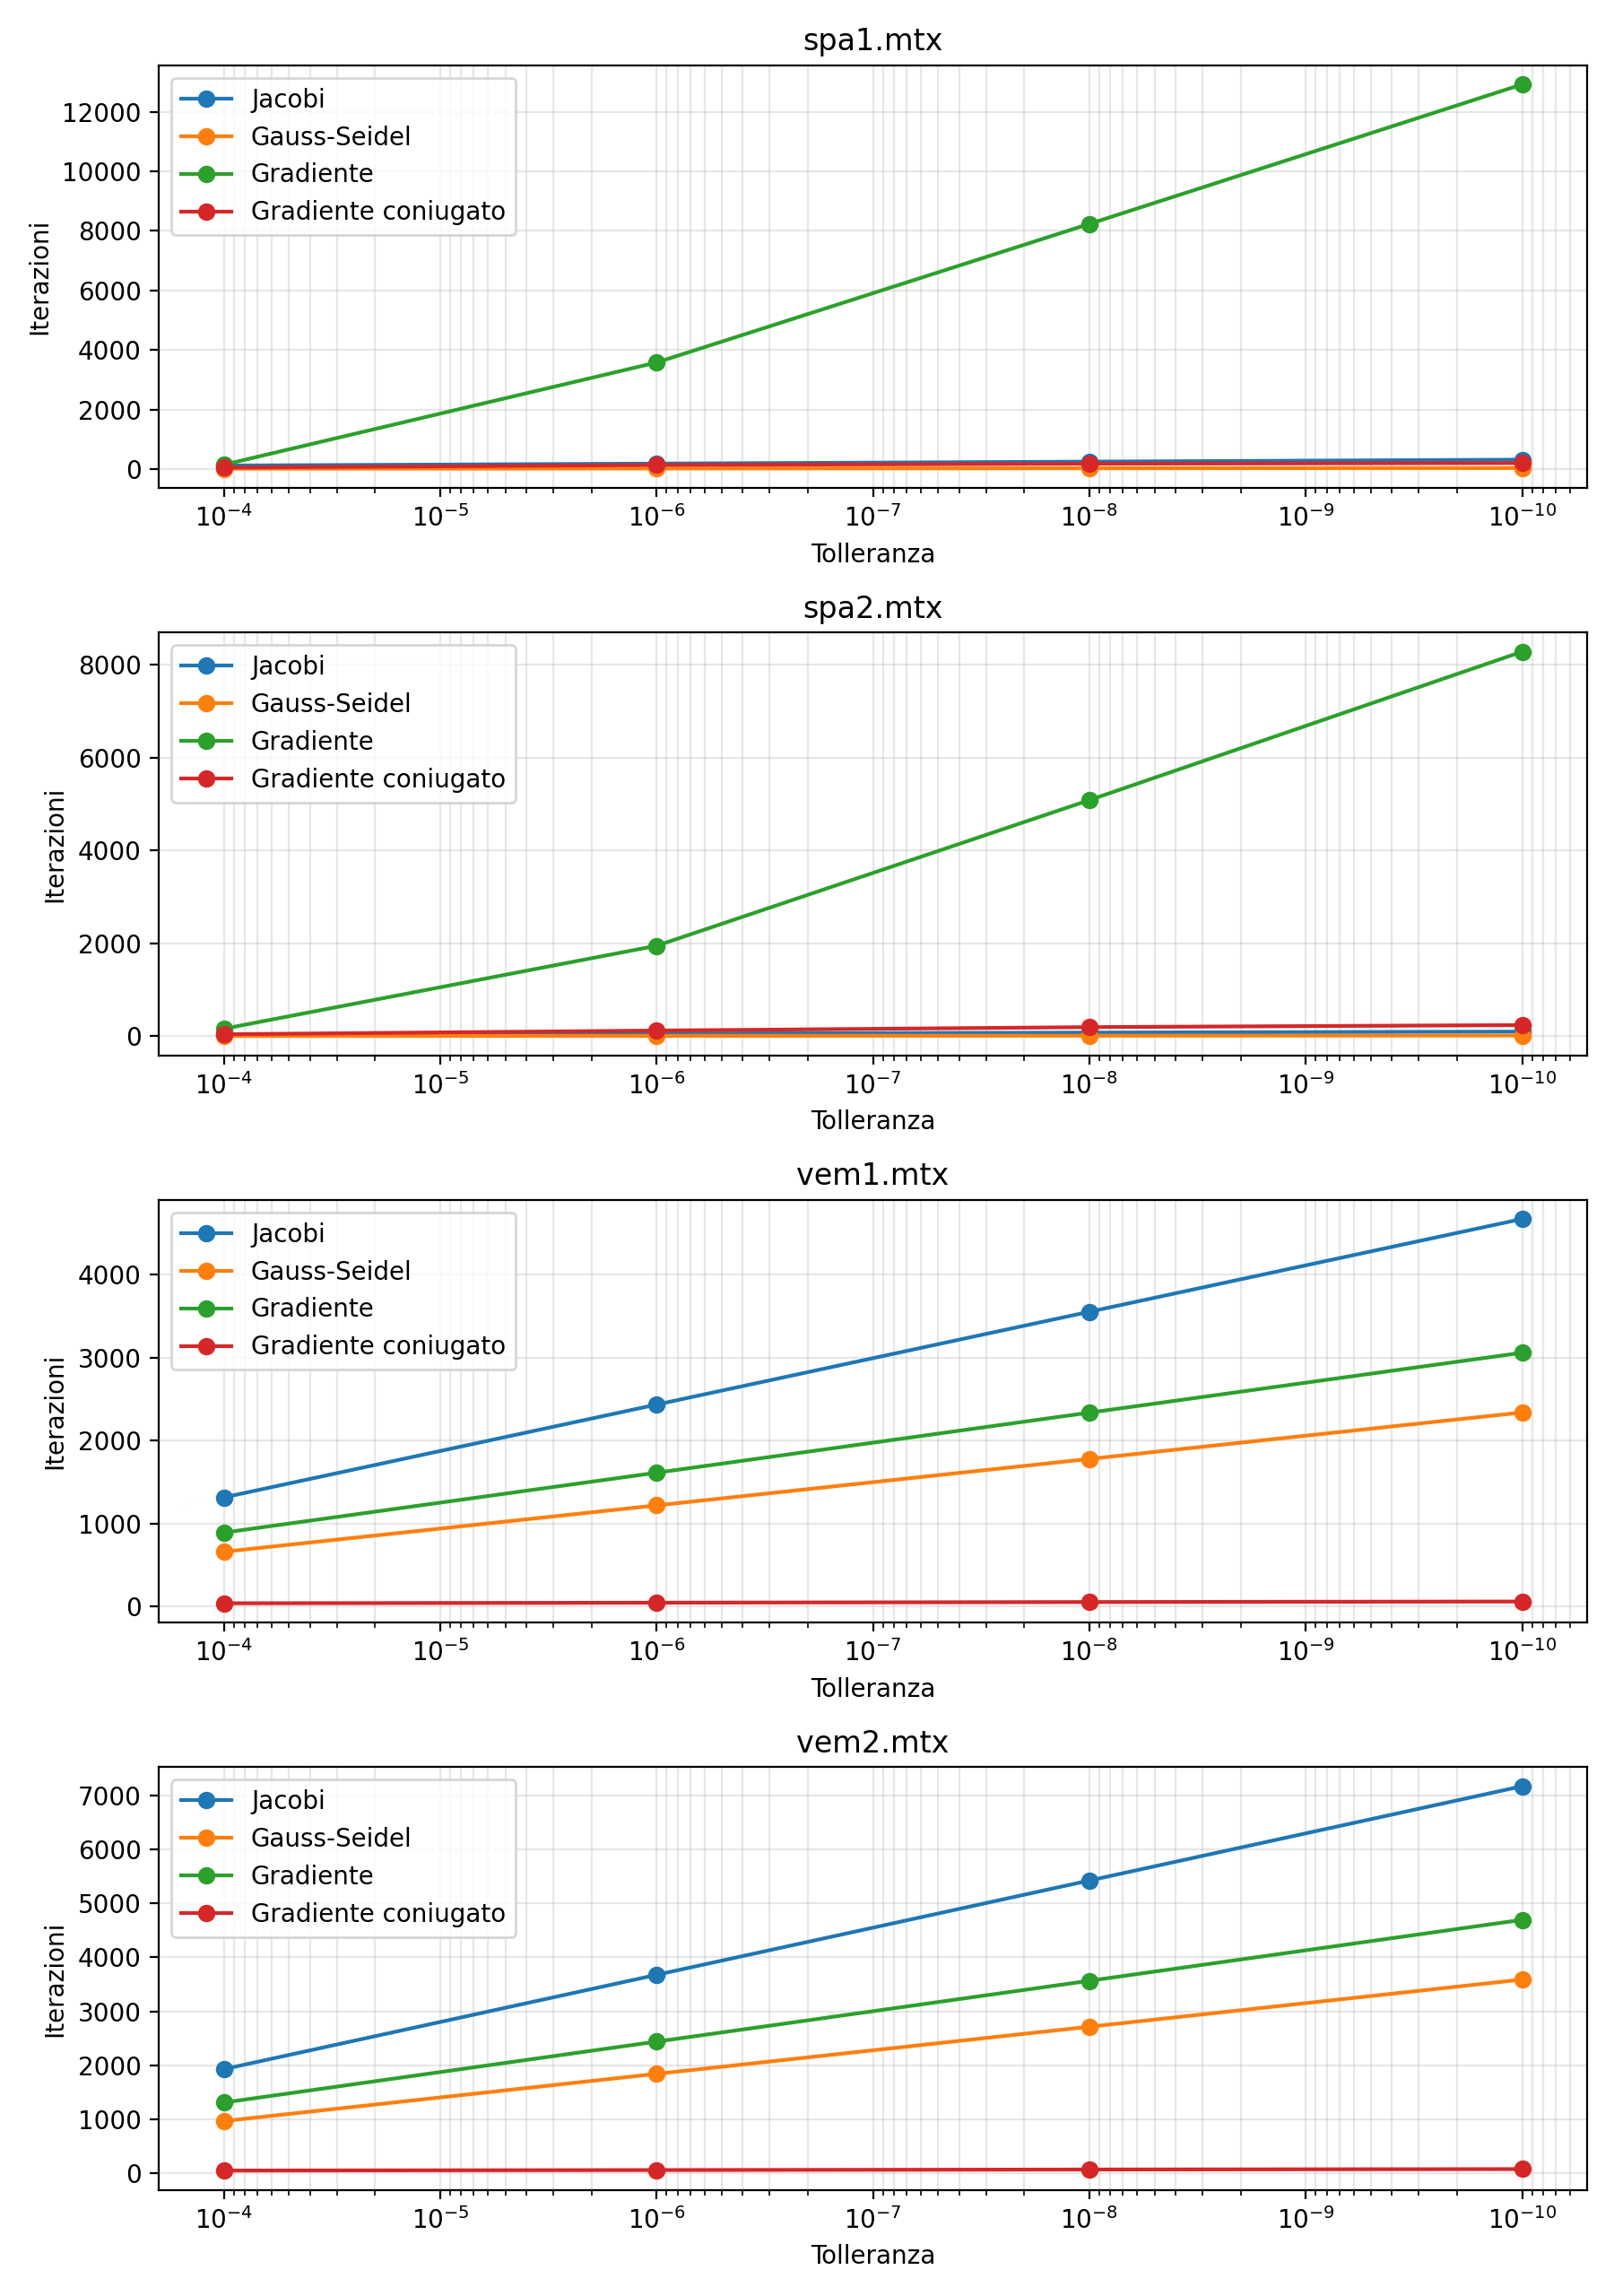
\includegraphics{../results/plots/iterations.png}}

\begin{frame}{Numero di iterazioni per tolleranza 1}
    \begin{figure}
        \centering
        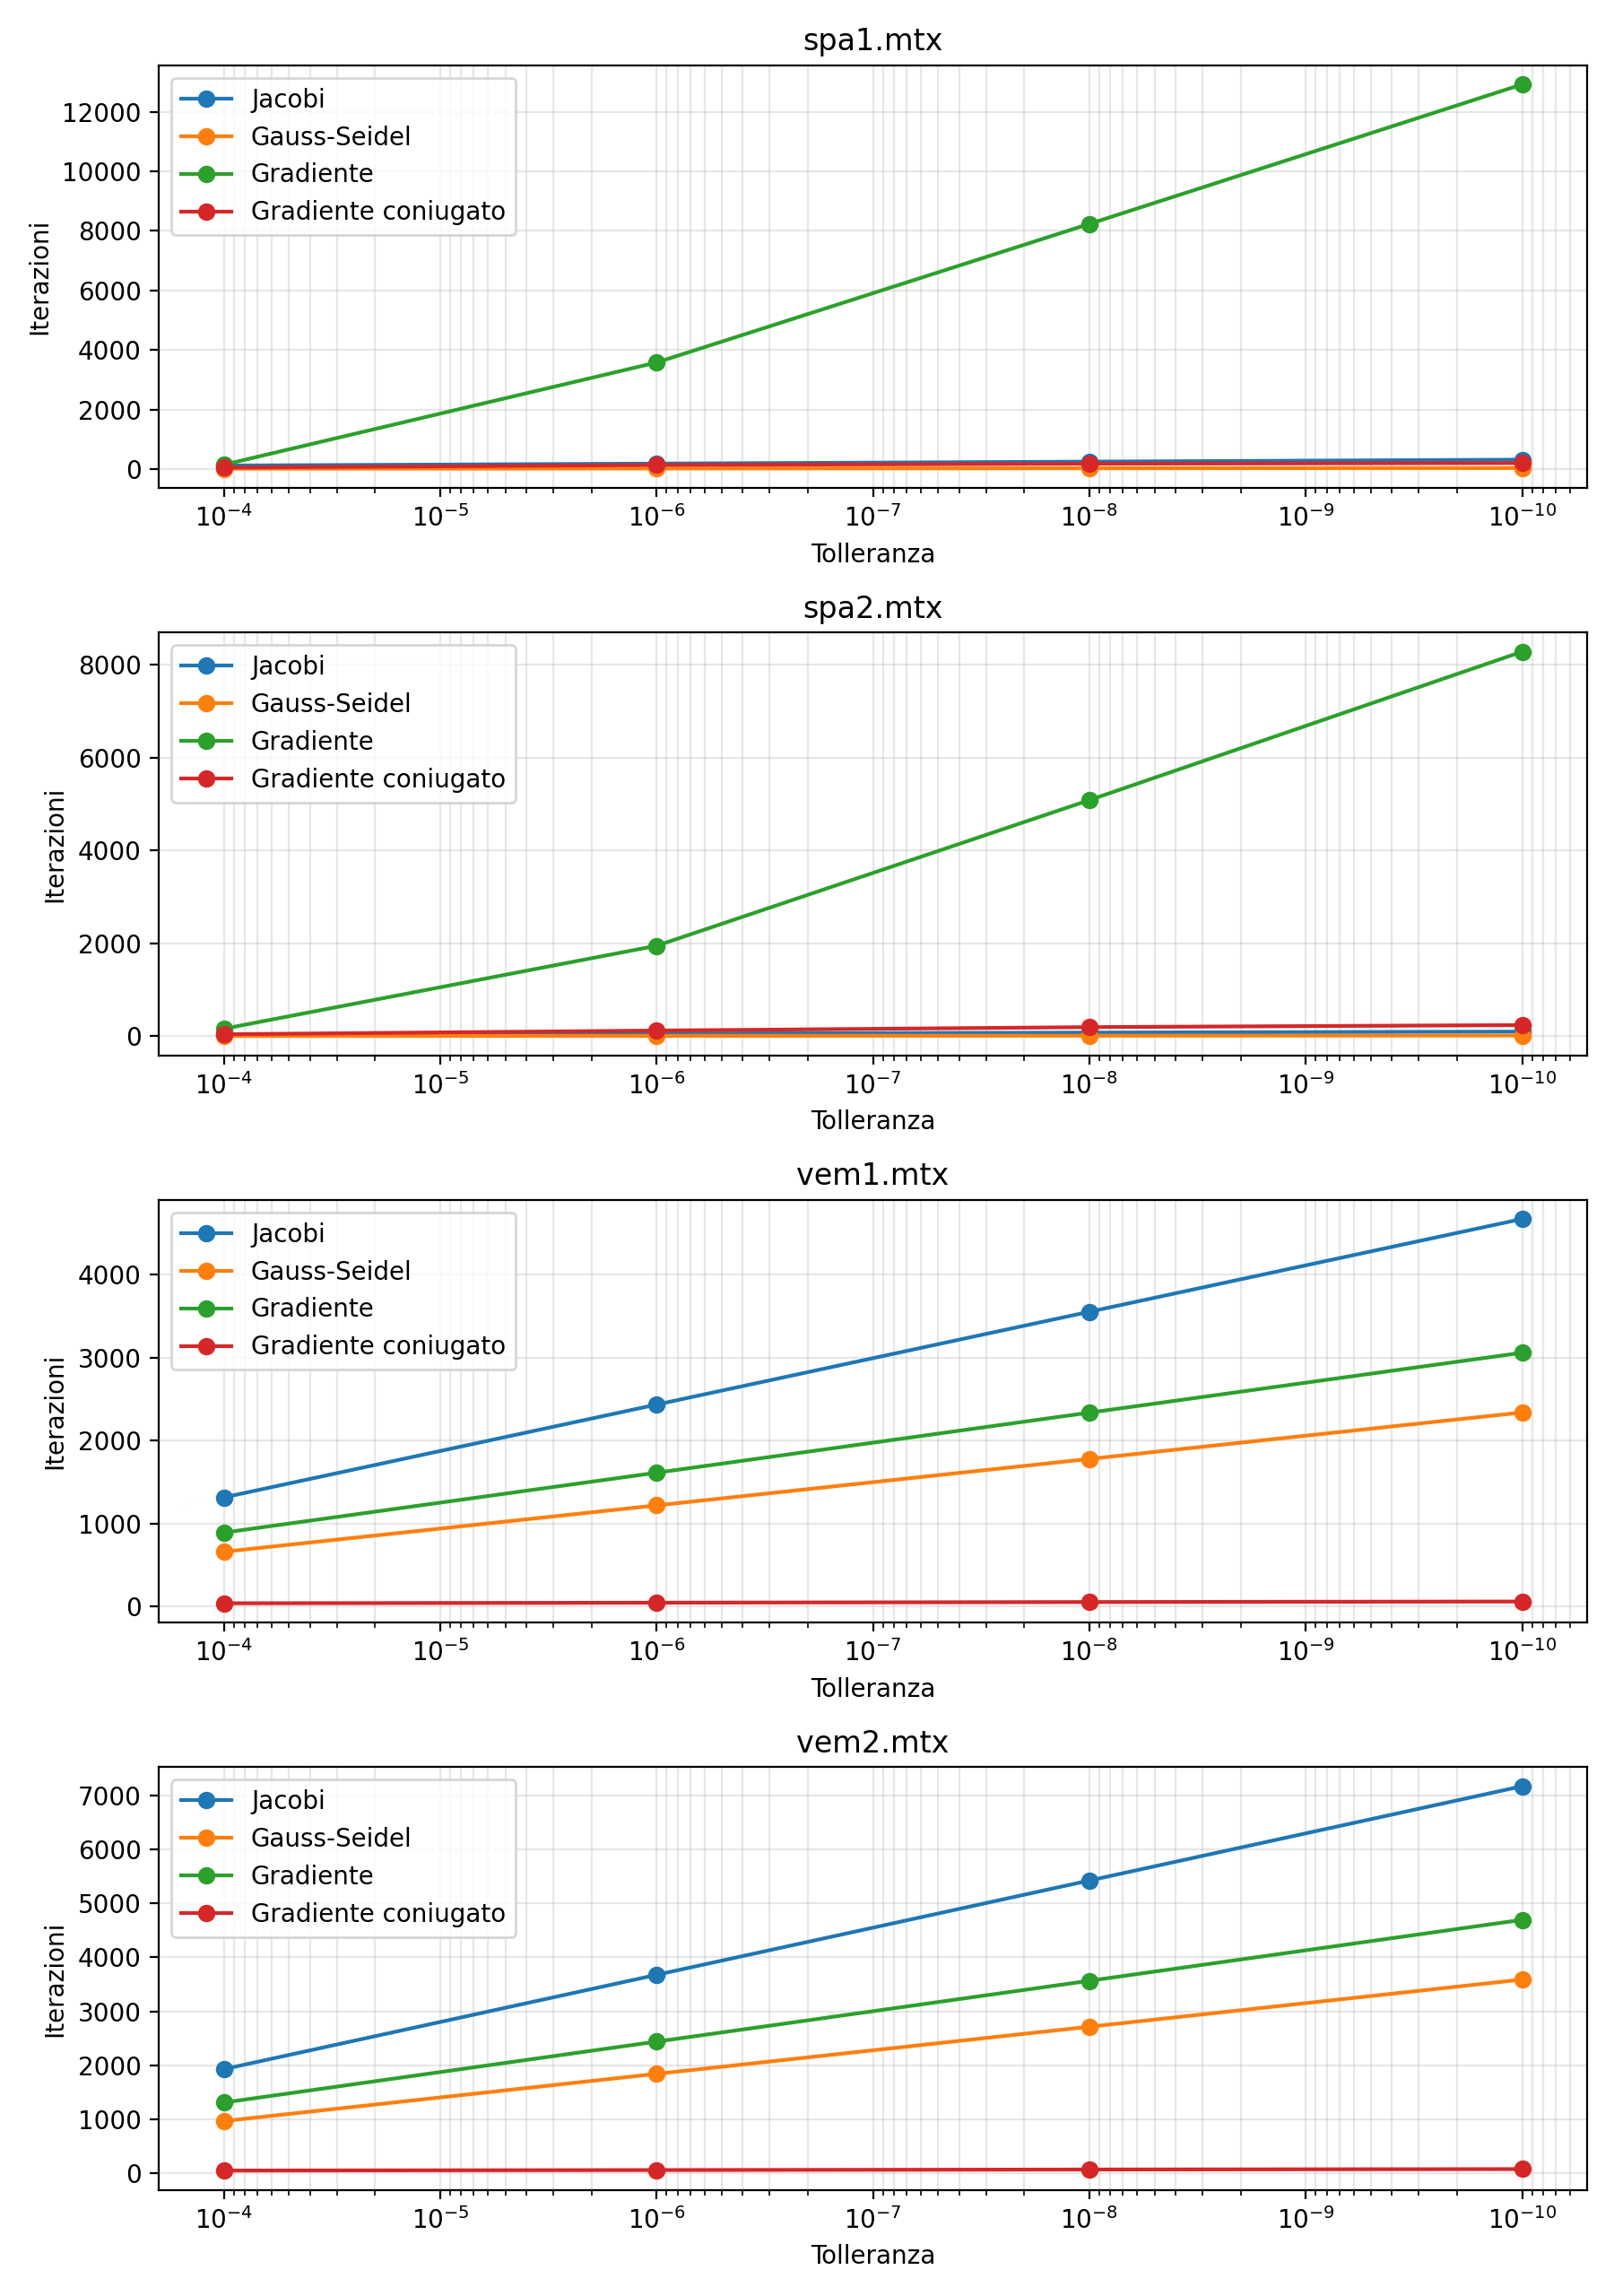
\includegraphics[trim=0pt {0.5\ht\iterbox} 0pt 0pt, clip, width=\textwidth, height=0.85\textheight, keepaspectratio]{../results/plots/iterations.png}
    \end{figure}
\end{frame}

\begin{frame}{Numero di iterazioni per tolleranza 2}
    \begin{figure}
        \centering
        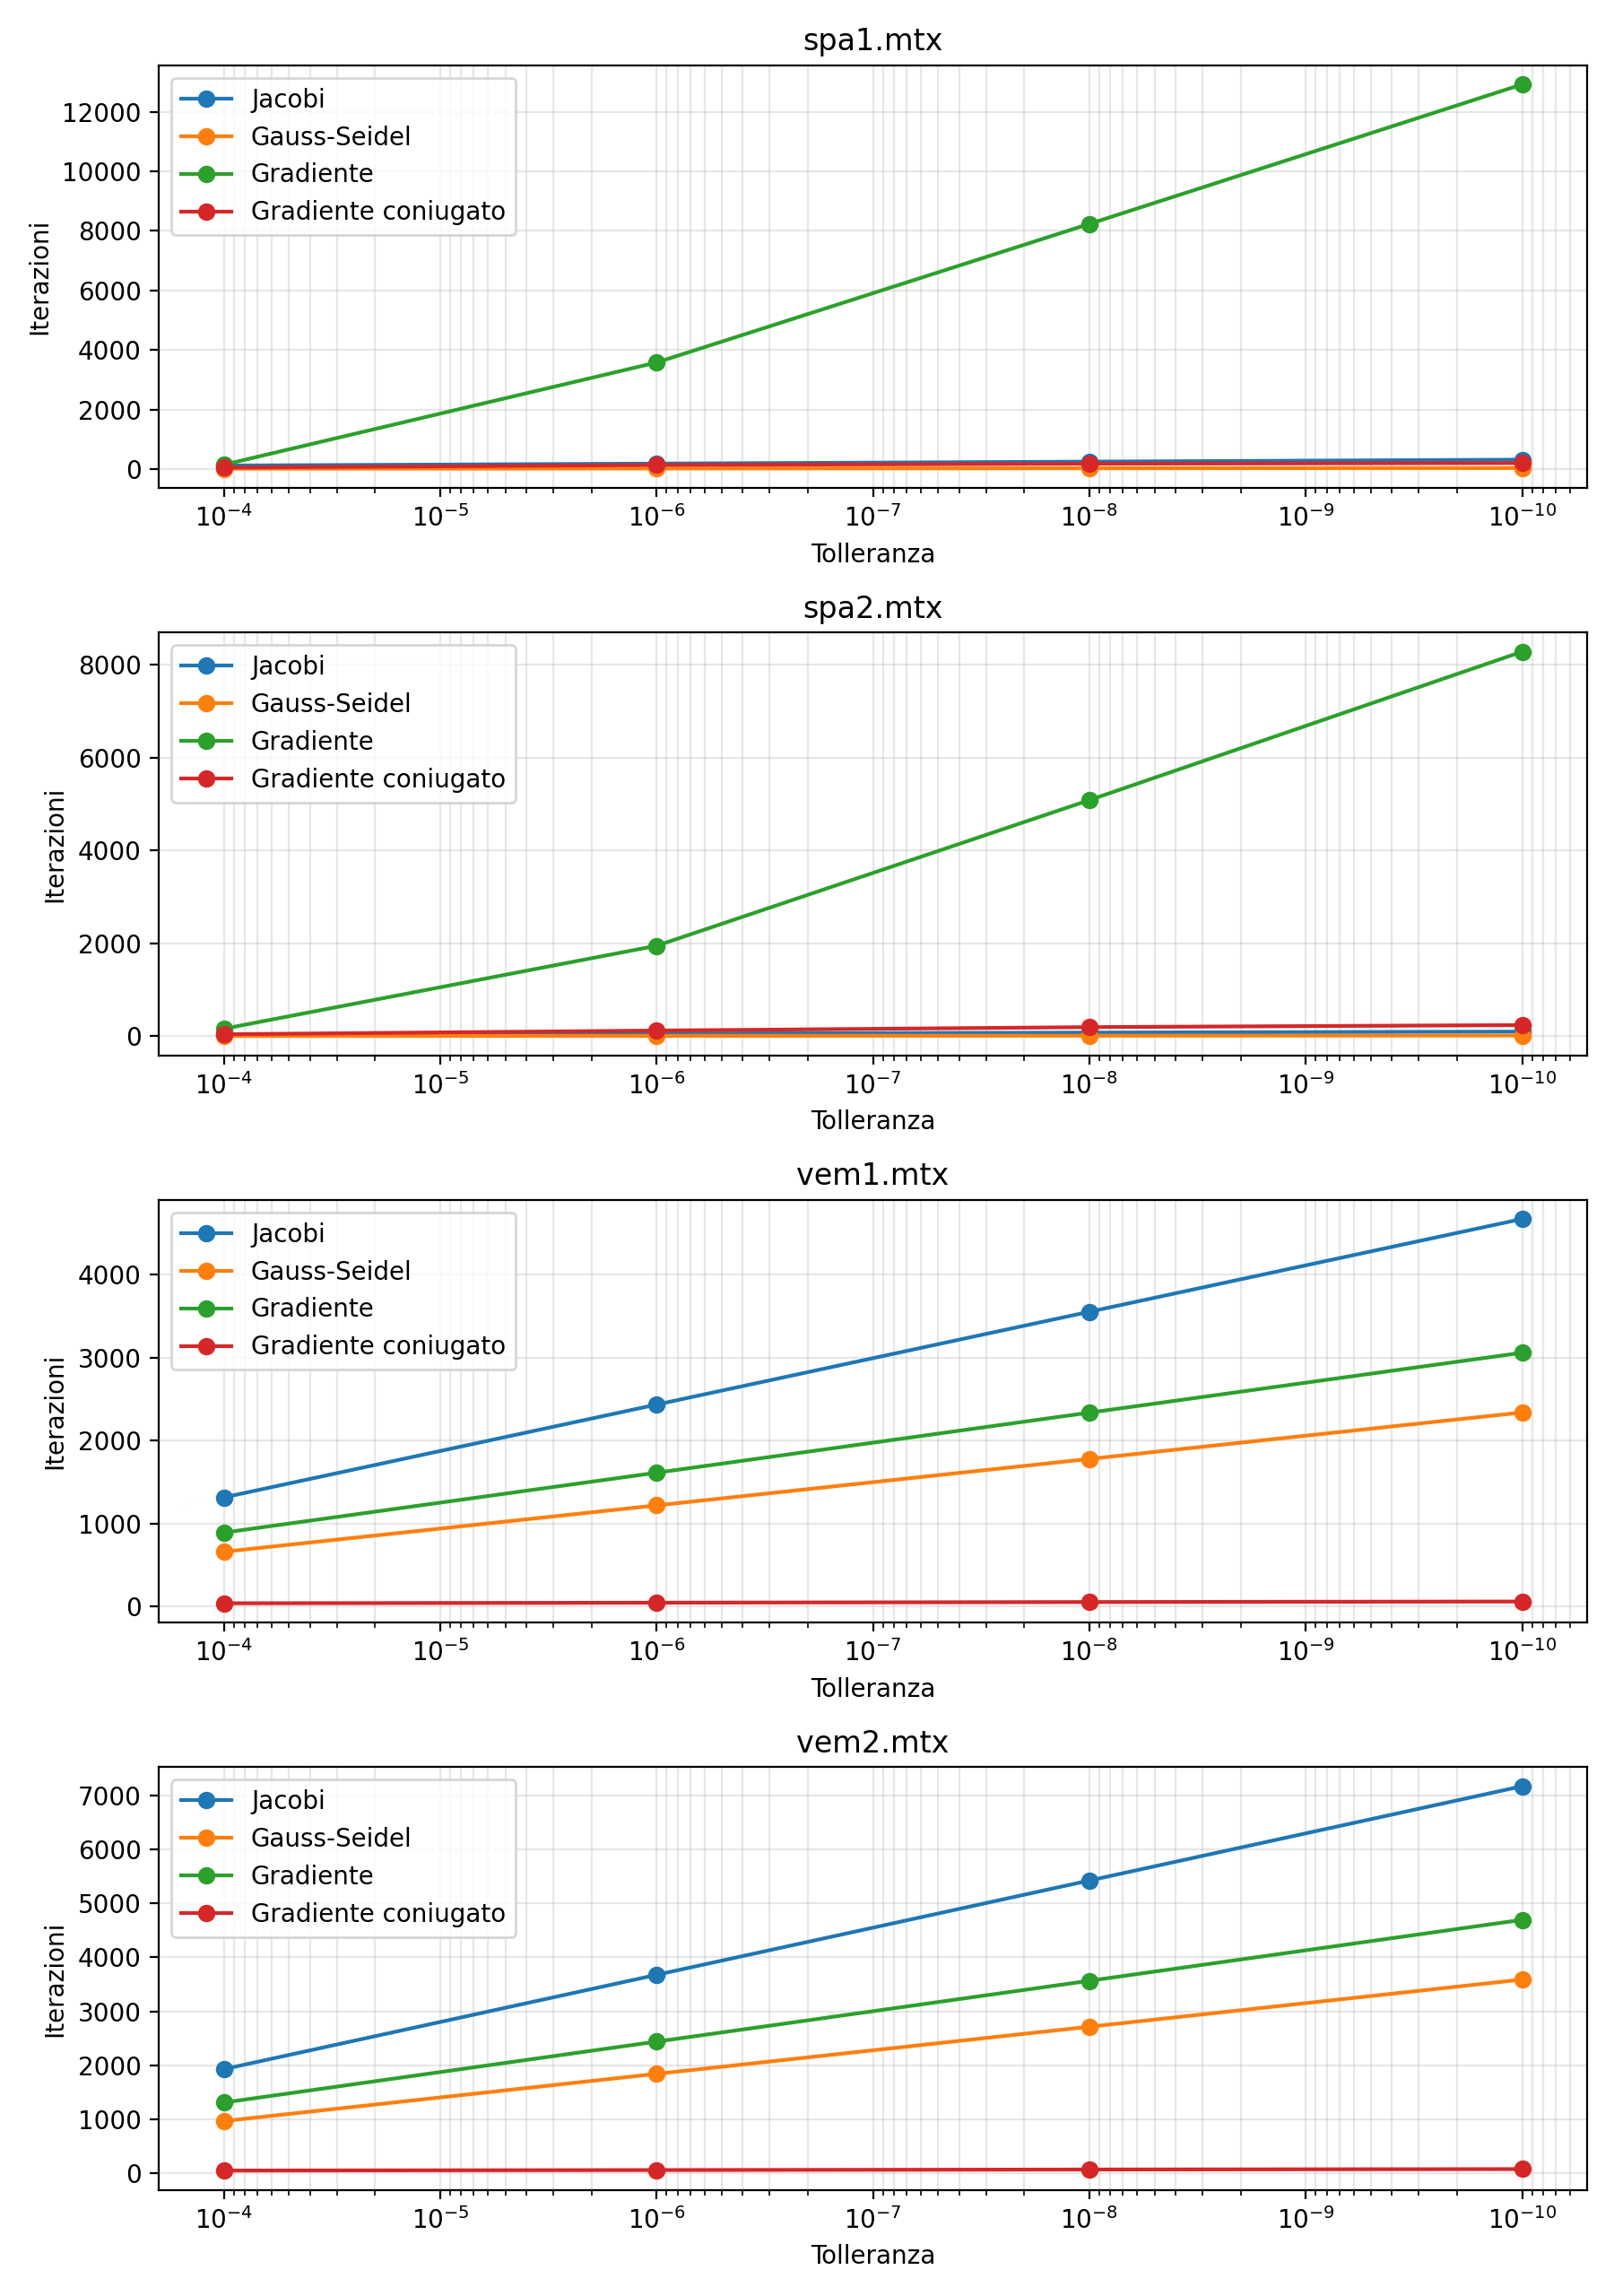
\includegraphics[trim=0pt 0pt 0pt {0.5\ht\iterbox}, clip, width=\textwidth, height=0.85\textheight, keepaspectratio]{../results/plots/iterations.png}
    \end{figure}
\end{frame}

\newsavebox{\errbox}
\sbox{\errbox}{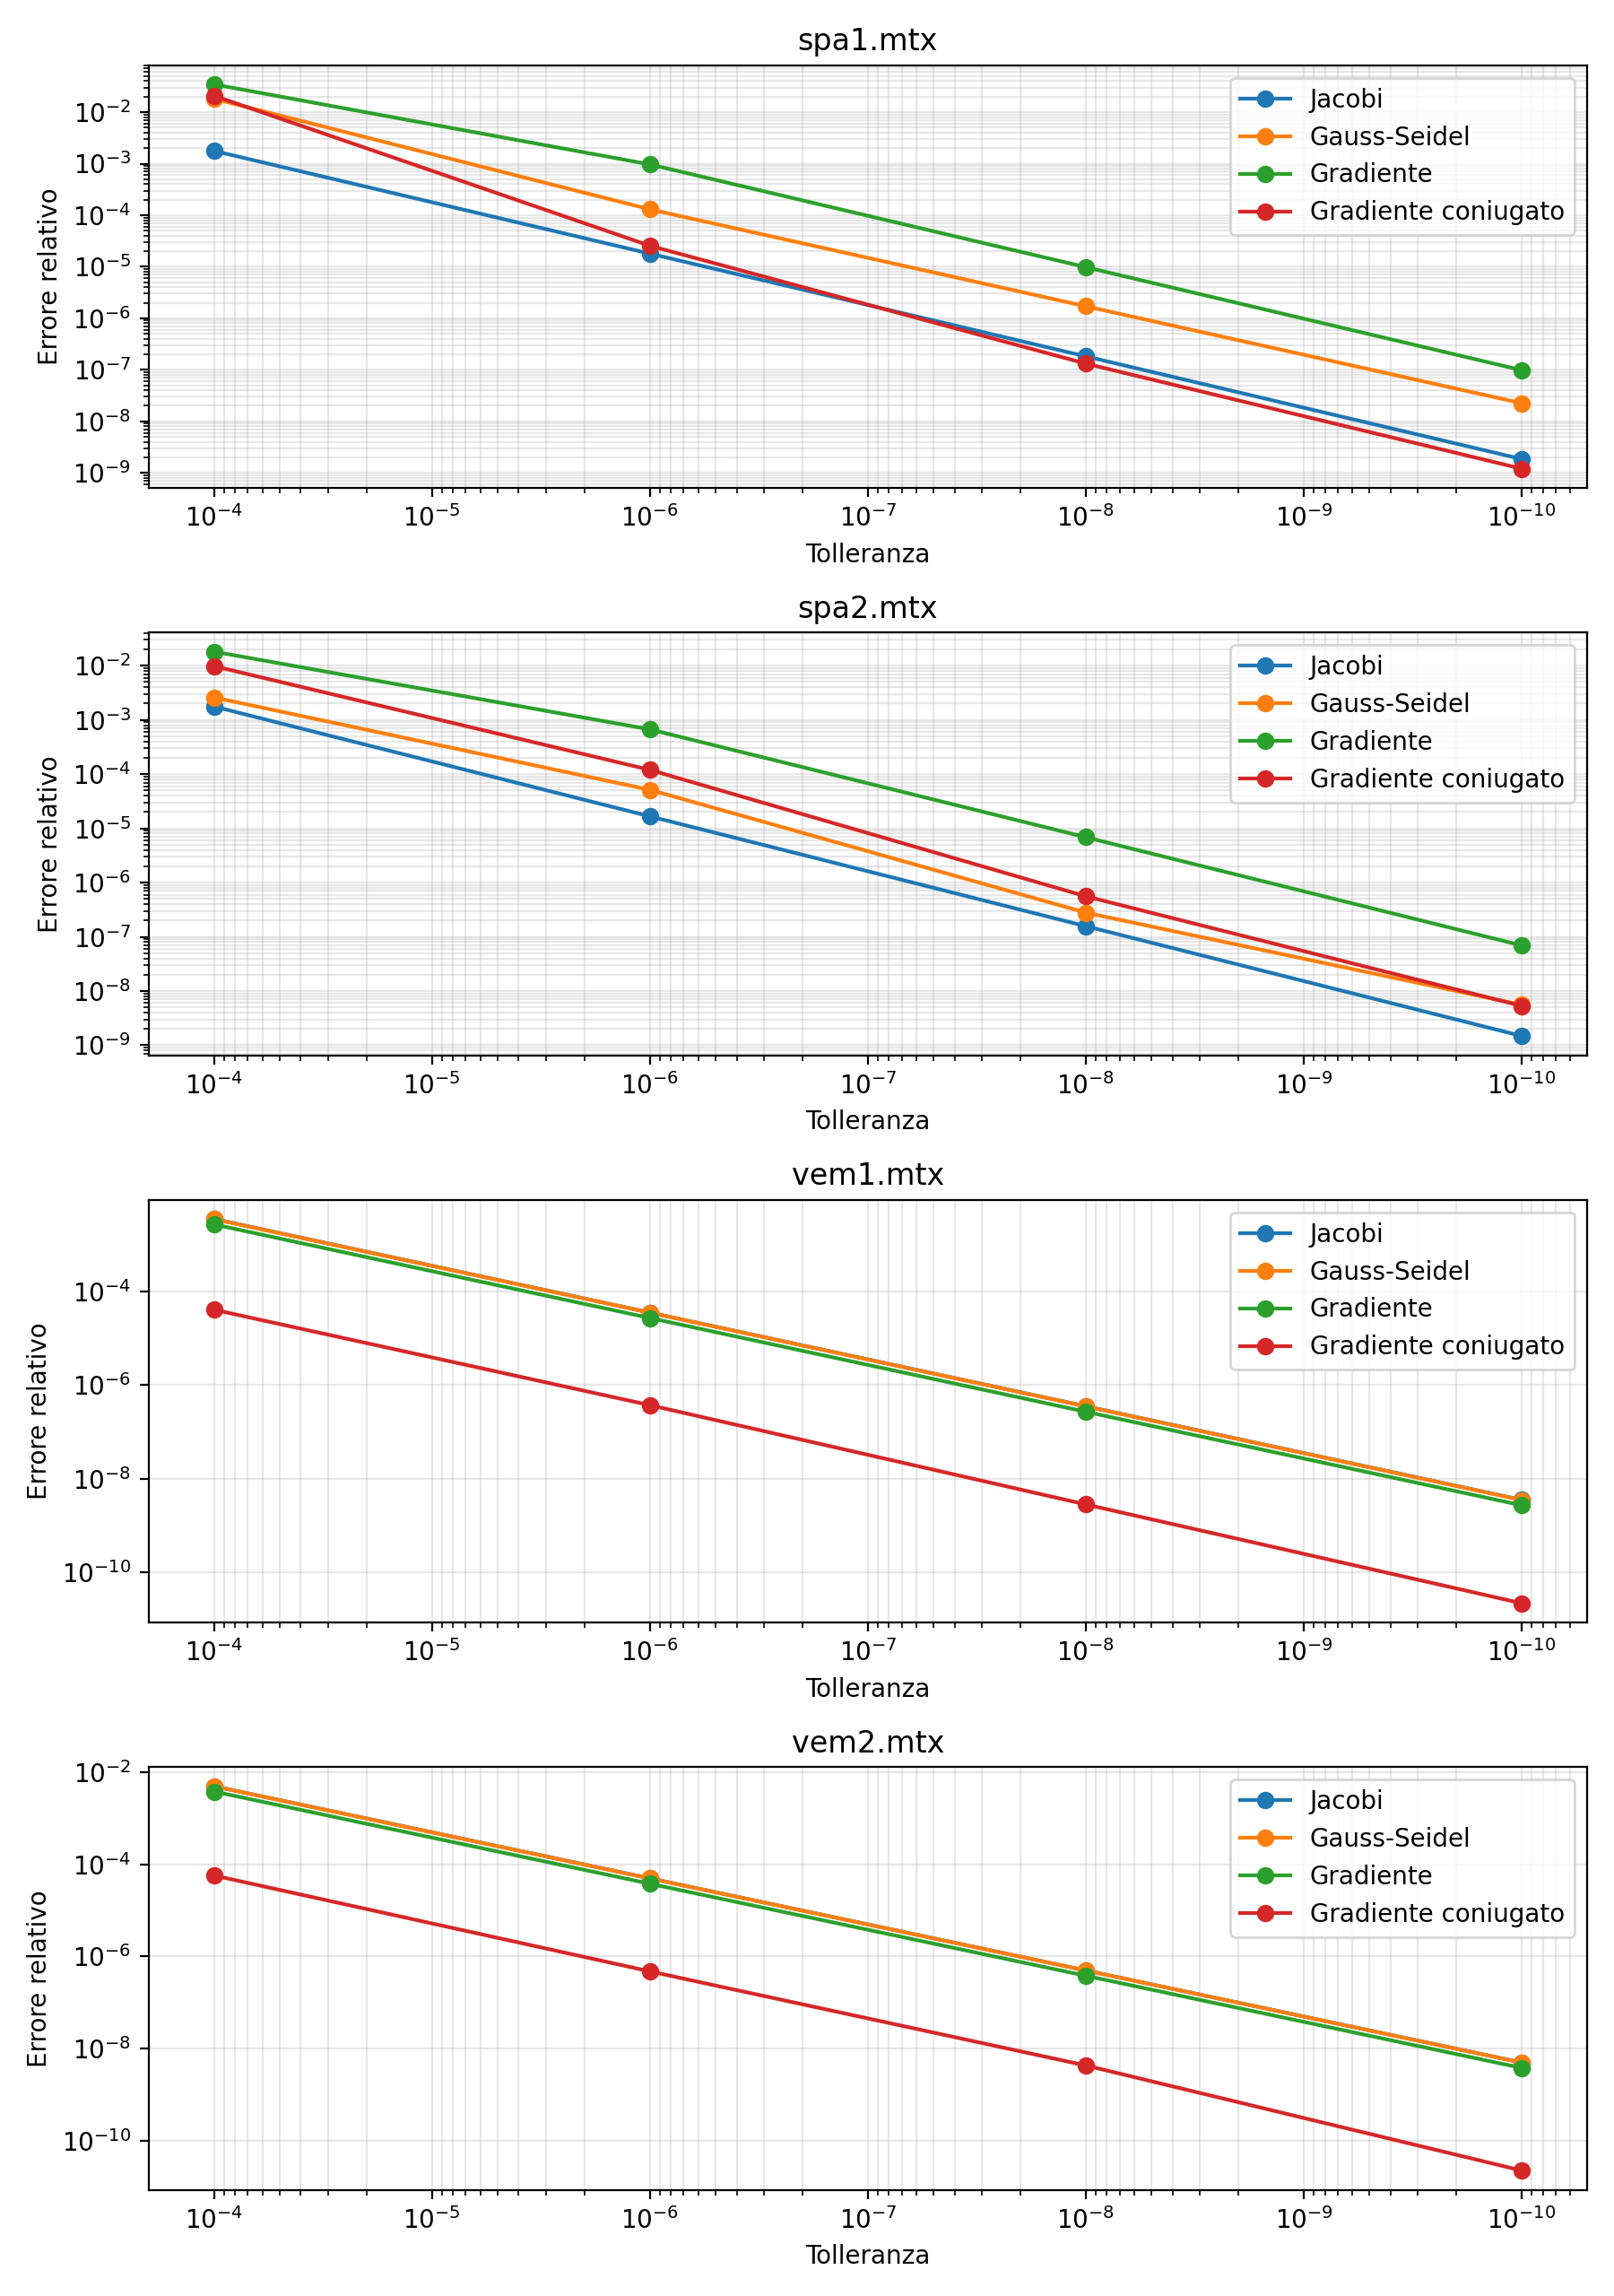
\includegraphics{../results/plots/relative_error.png}}

\begin{frame}{Errore relativo misurato 1}
    \begin{figure}
        \centering
        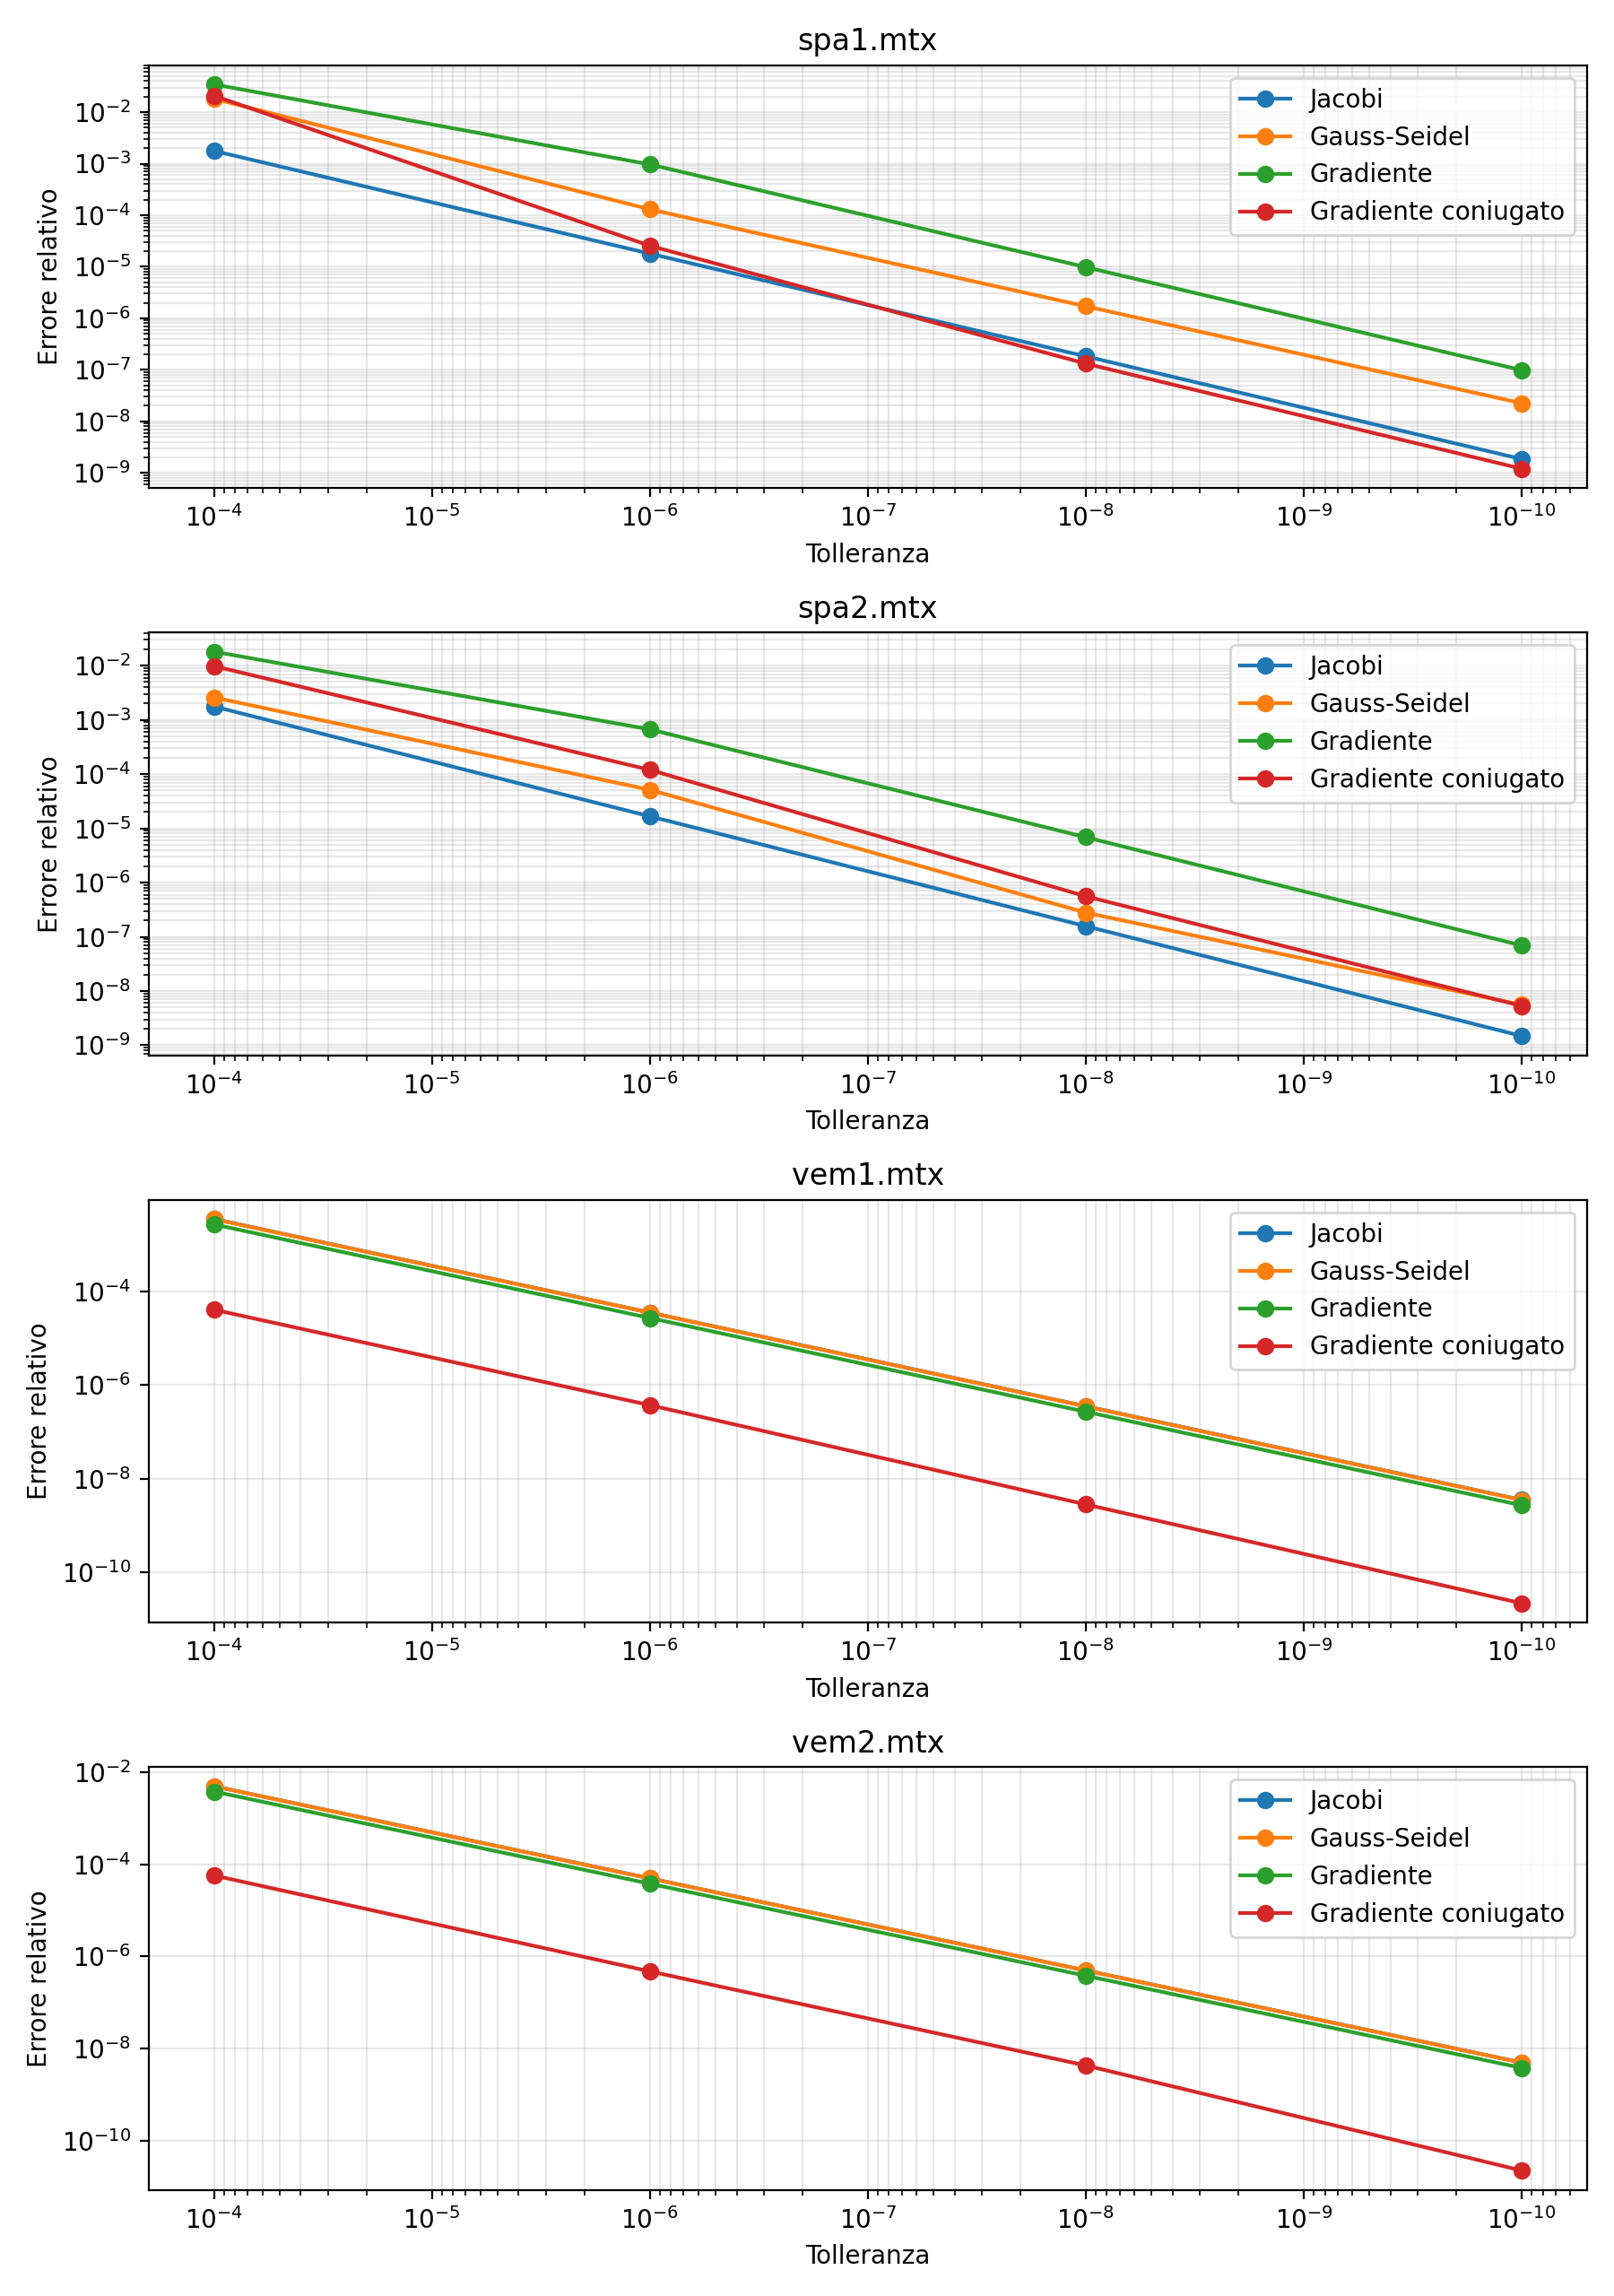
\includegraphics[trim=0pt {0.5\ht\errbox} 0pt 0pt, clip, width=\textwidth, height=0.85\textheight, keepaspectratio]{../results/plots/relative_error.png}
    \end{figure}
\end{frame}

\begin{frame}{Errore relativo misurato 2}
    \begin{figure}
        \centering
        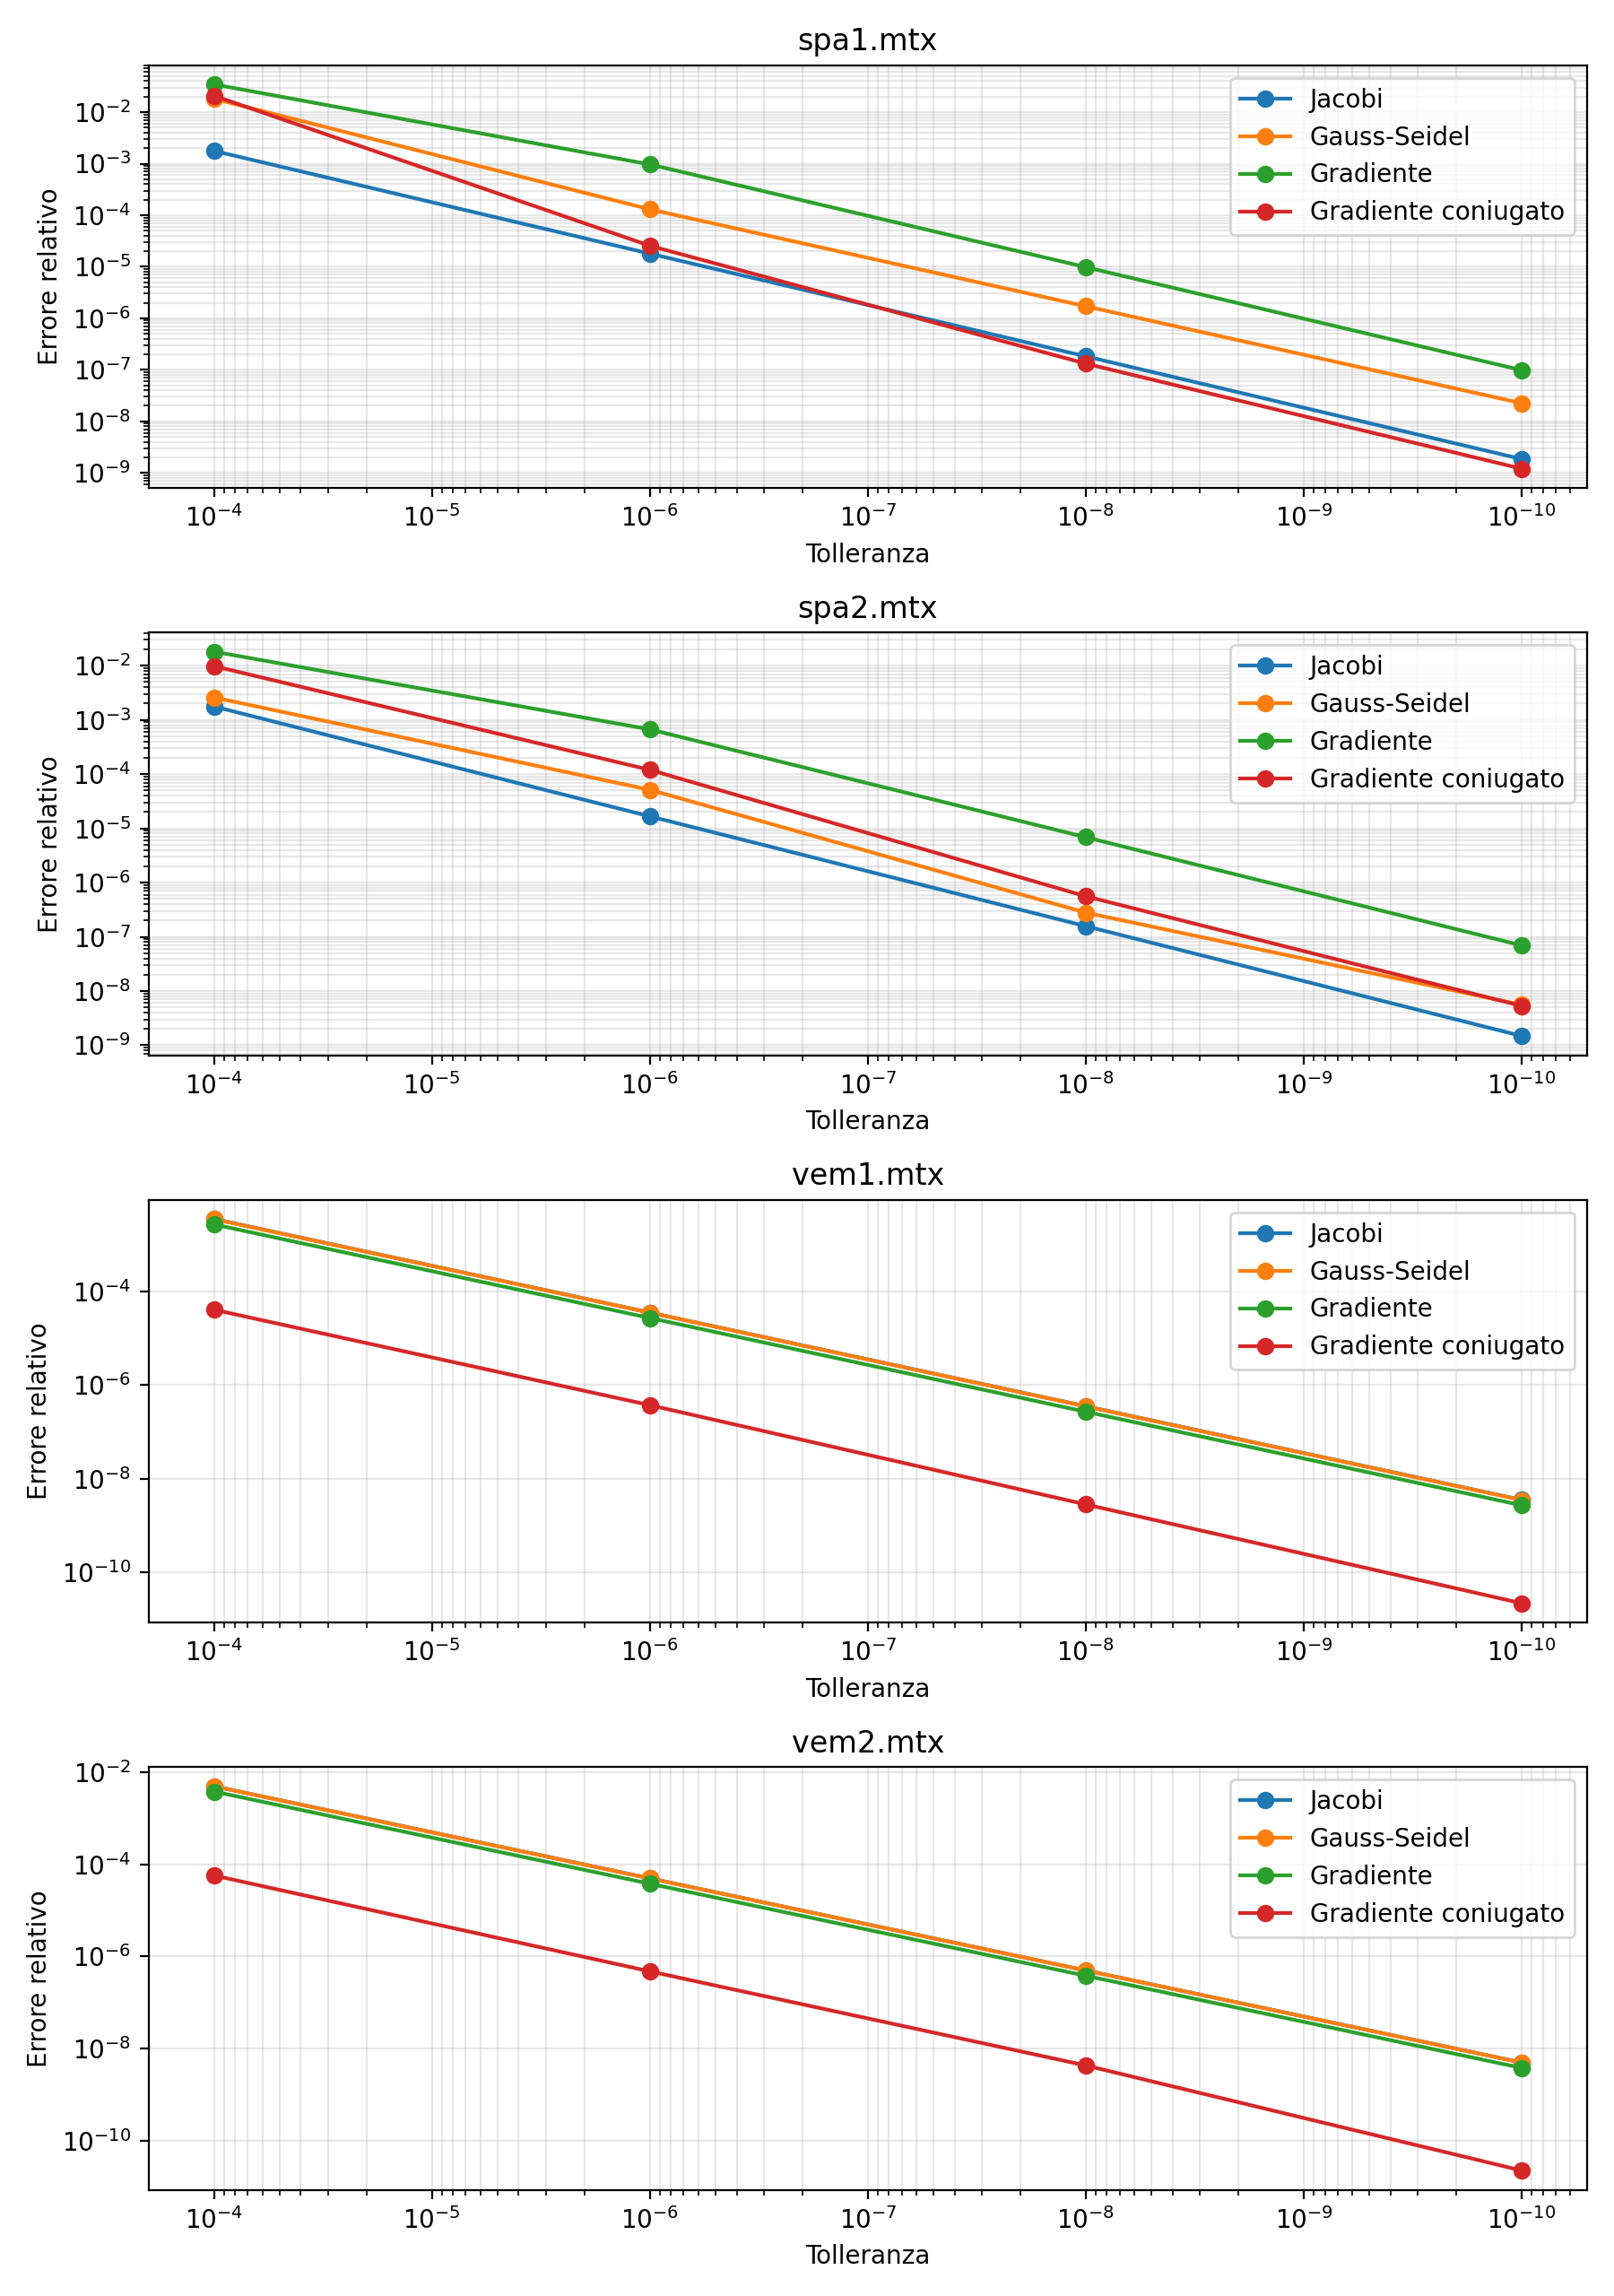
\includegraphics[trim=0pt 0pt 0pt {0.5\ht\errbox}, clip, width=\textwidth, height=0.85\textheight, keepaspectratio]{../results/plots/relative_error.png}
    \end{figure}
\end{frame}

\begin{frame}{Tempi totali di calcolo}
    \begin{itemize}
        \item \textbf{Sulle matrici \texttt{spa}:} il più veloce è Gauss-Seidel, perché converge in pochissime iterazioni e questo compensa il costo del passo sequenziale.
        \item \textbf{Sulle matrici \texttt{vem}:} la situazione si ribalta, e il gradiente coniugato è di gran lunga il più veloce (frazioni di millisecondo), staccando nettamente gli altri tre.
        \item \textbf{Gradiente semplice:} si conferma di gran lunga il più lento, in particolare sulle \texttt{spa}, arrivando quasi a 10 secondi su \texttt{spa2}.
    \end{itemize}
\end{frame}

\newsavebox{\timebox}
\sbox{\timebox}{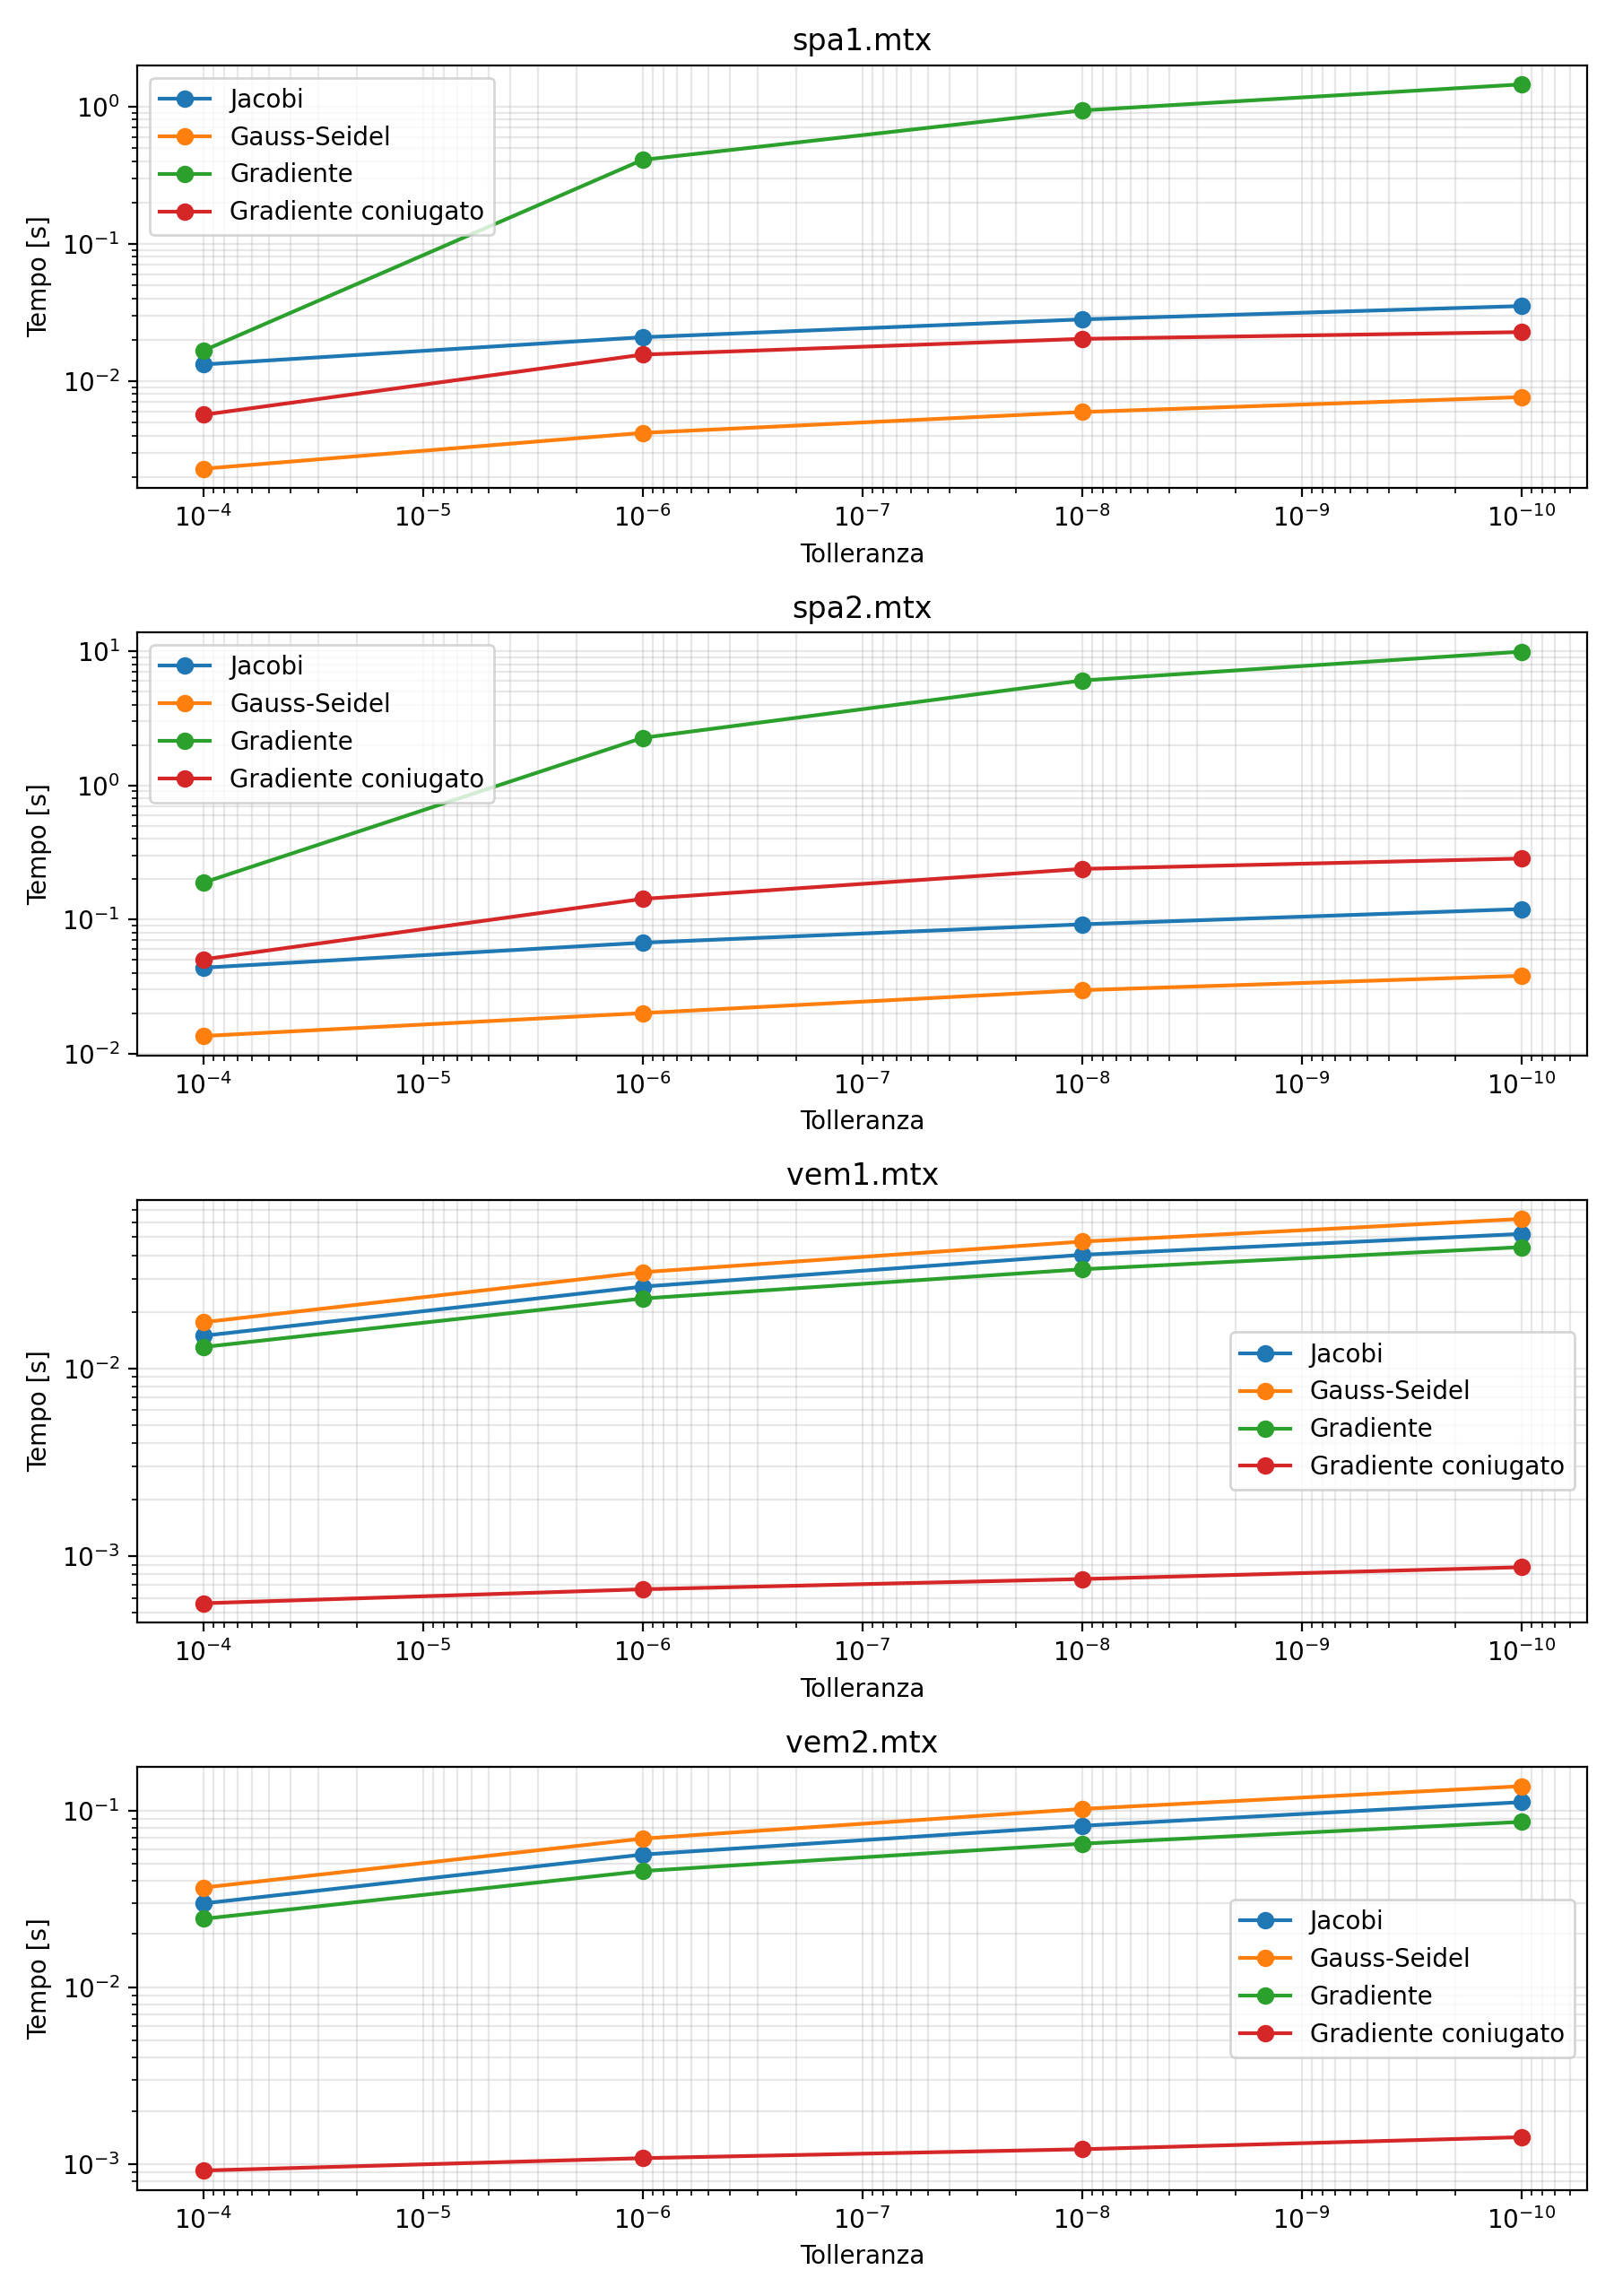
\includegraphics{../results/plots/time.png}}

\begin{frame}{Tempi totali di calcolo 1}
    \begin{figure}
        \centering
        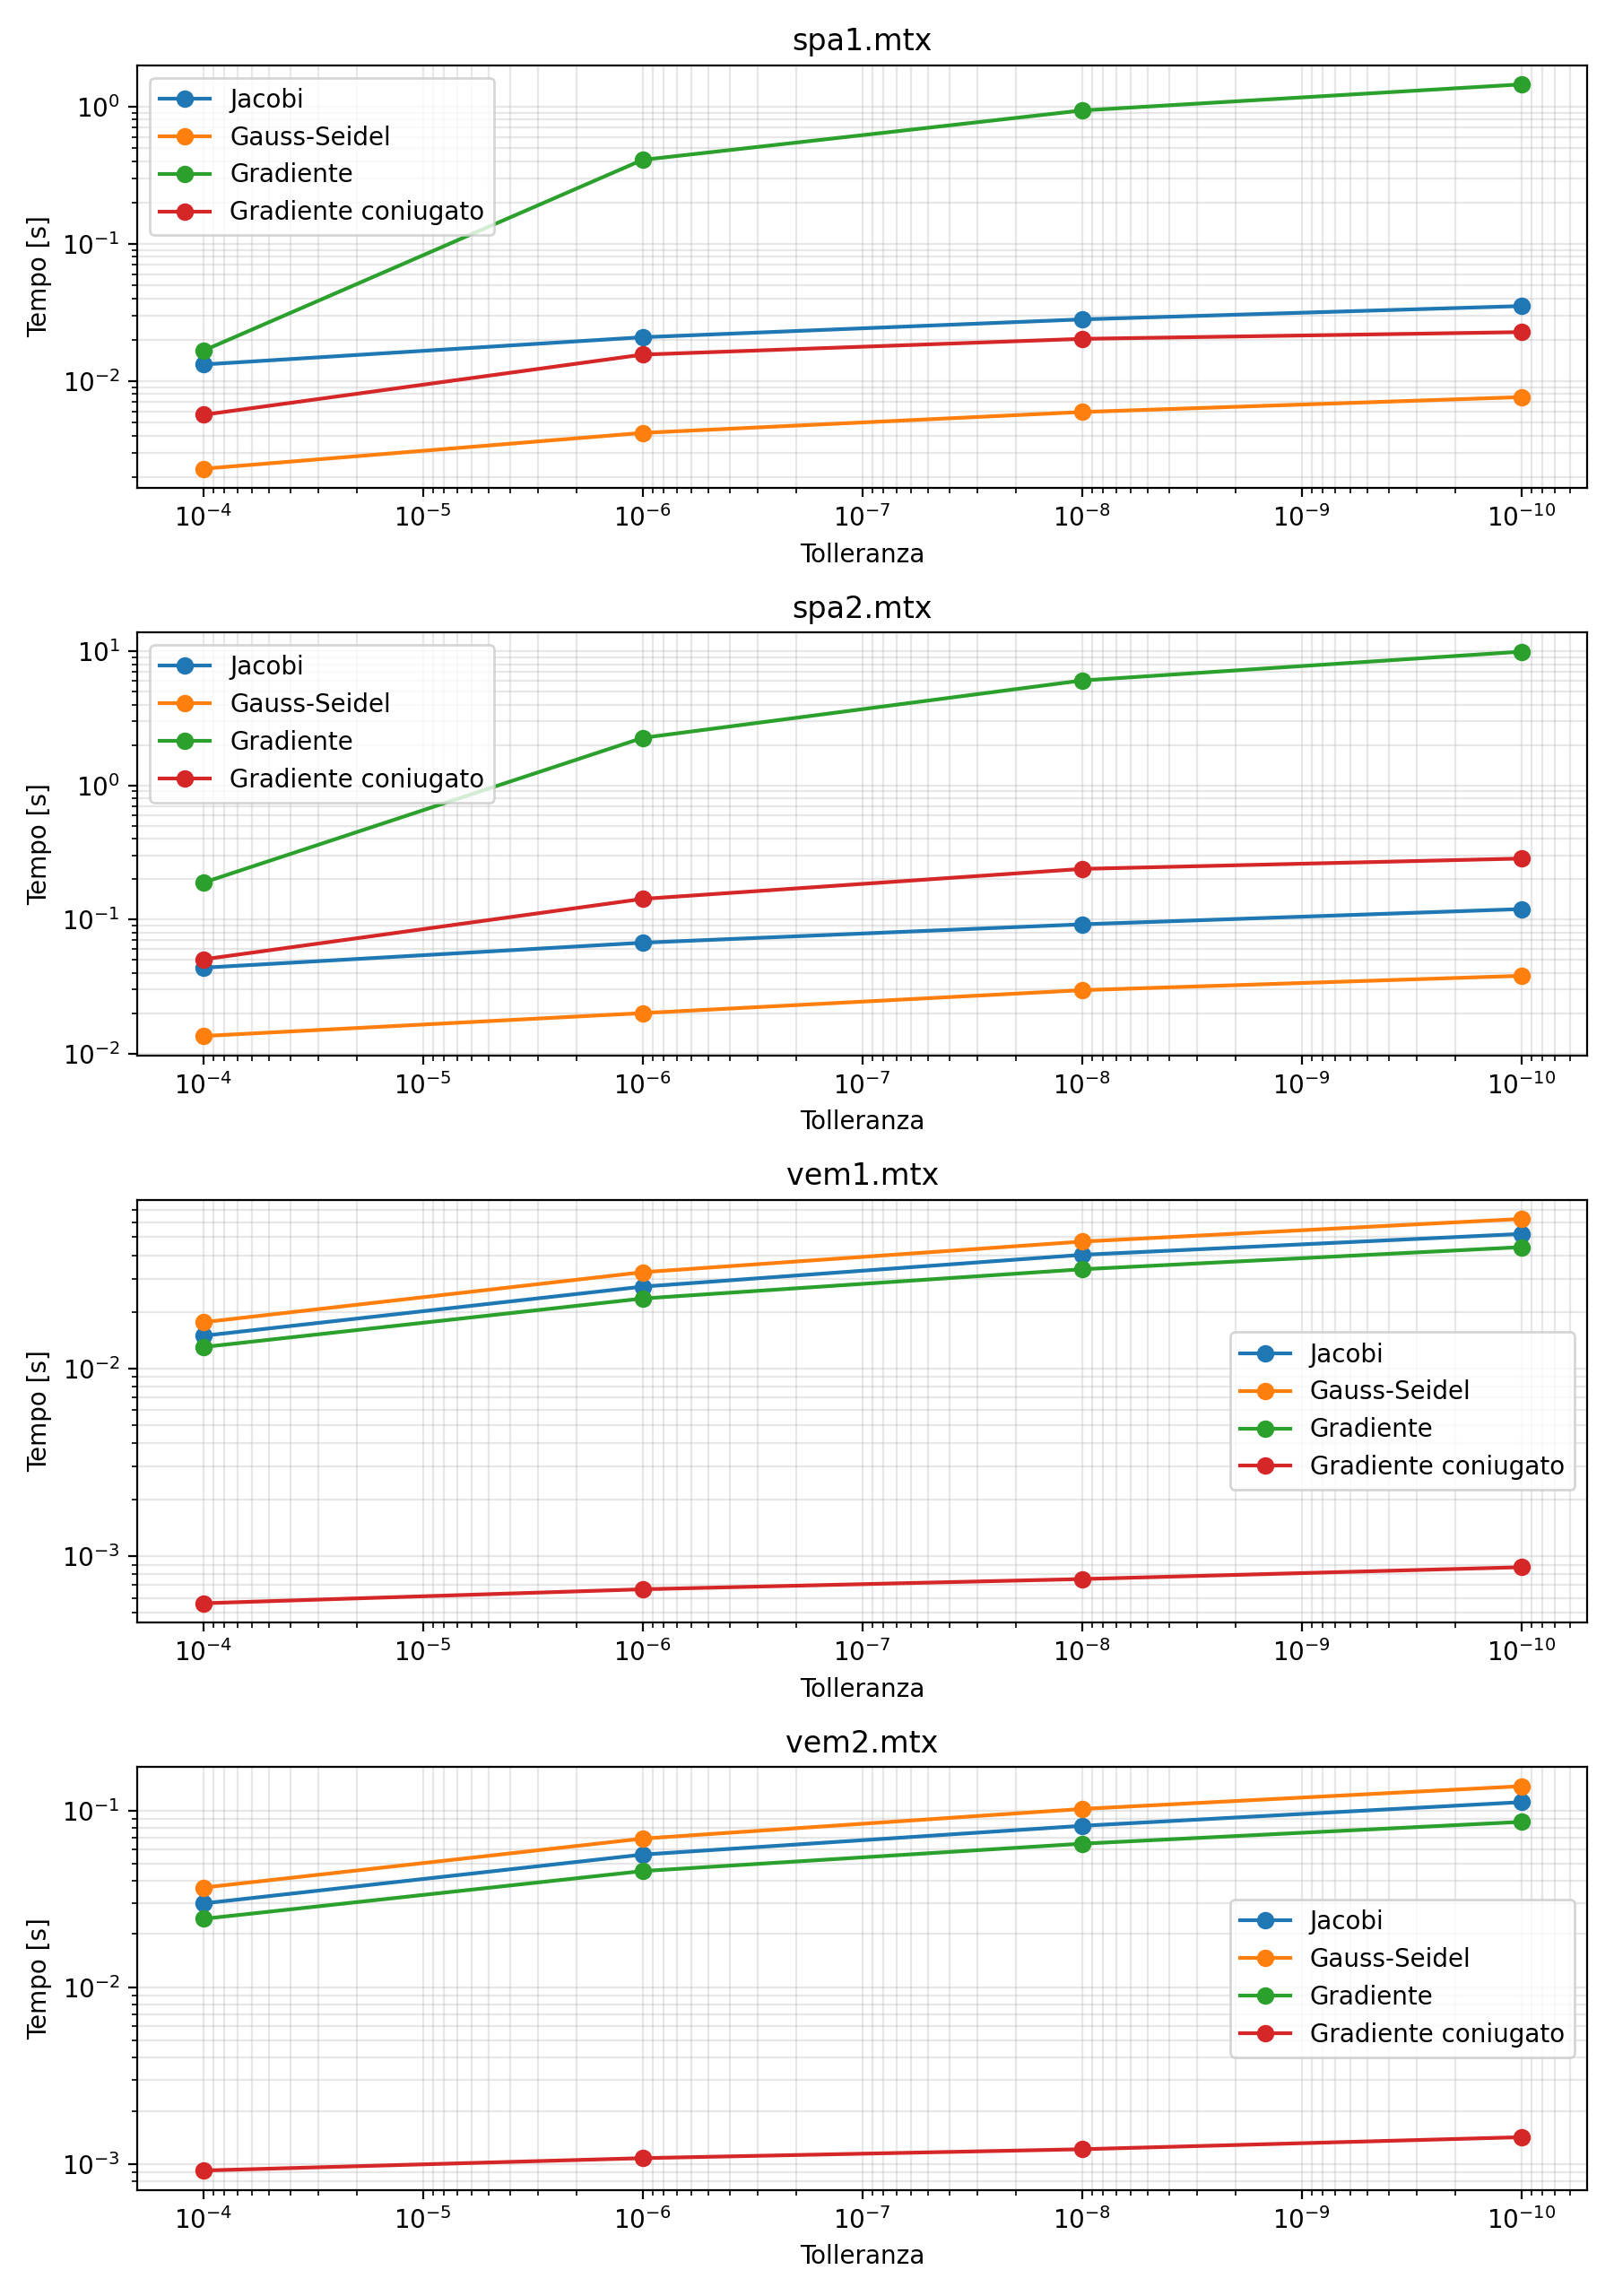
\includegraphics[trim=0pt {0.5\ht\timebox} 0pt 0pt, clip, width=\textwidth, height=0.85\textheight, keepaspectratio]{../results/plots/time.png}
    \end{figure}
\end{frame}

\begin{frame}{Tempi totali di calcolo 2}
    \begin{figure}
        \centering
        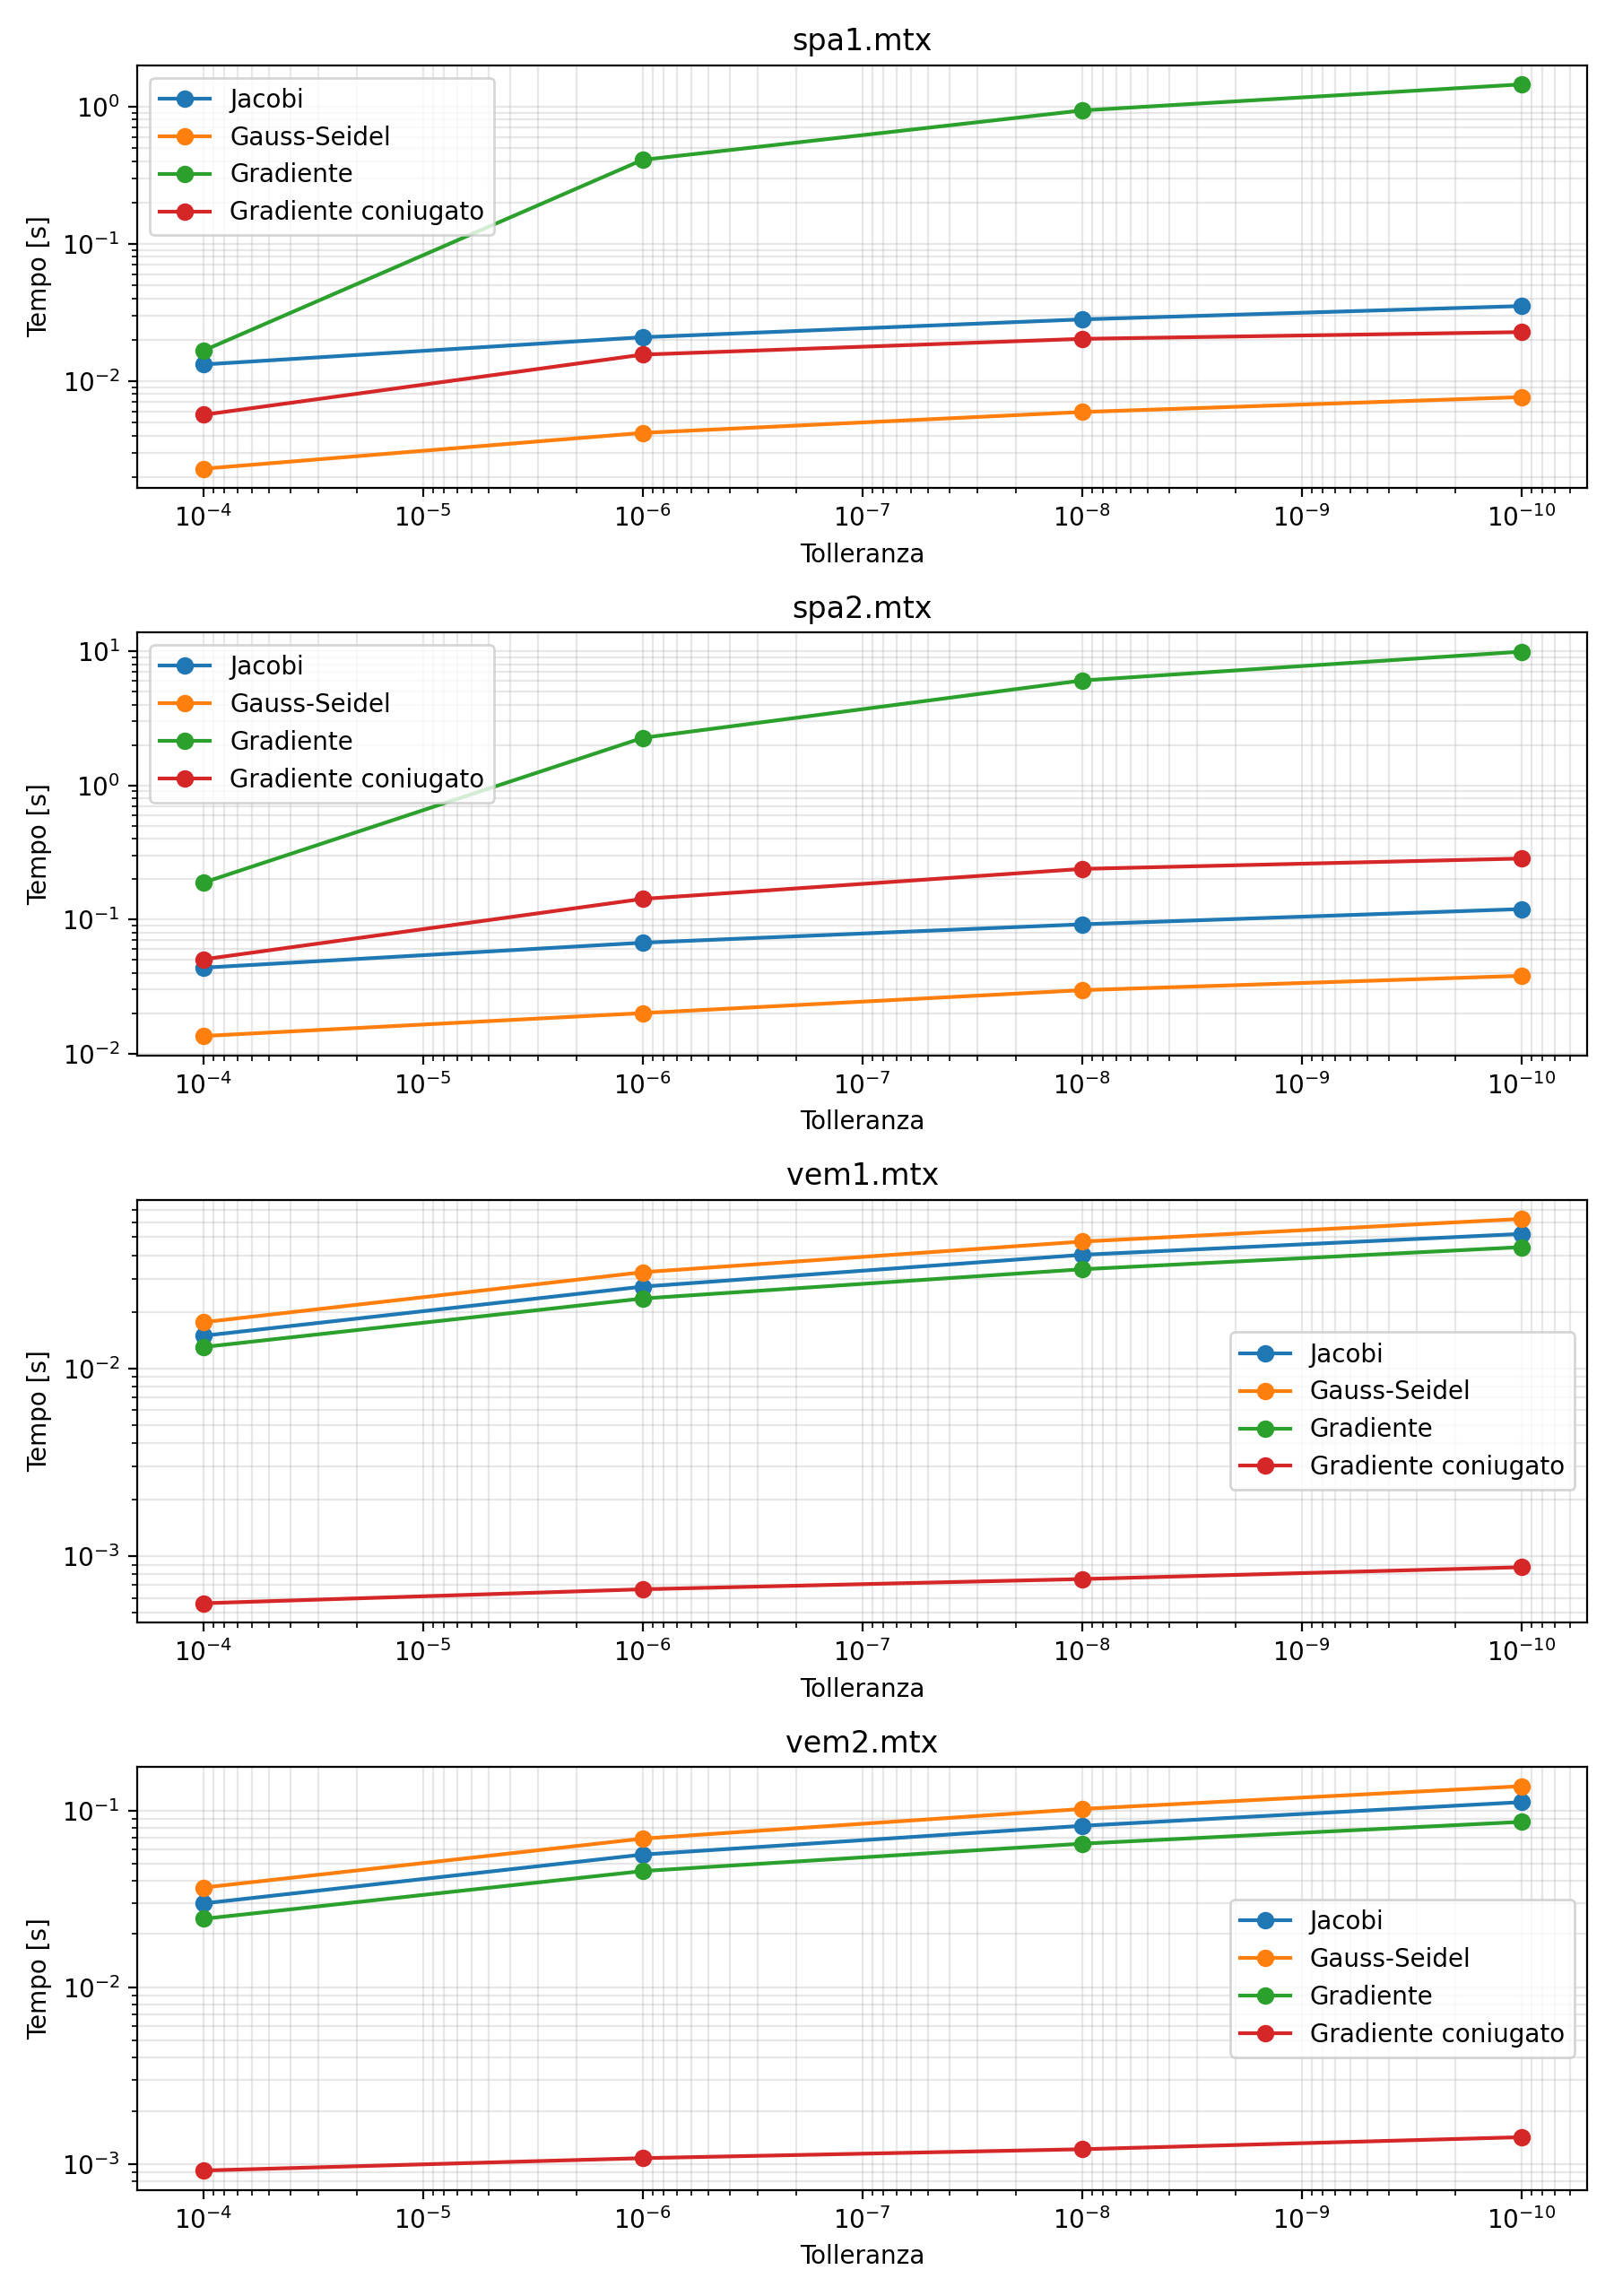
\includegraphics[trim=0pt 0pt 0pt {0.5\ht\timebox}, clip, width=\textwidth, height=0.85\textheight, keepaspectratio]{../results/plots/time.png}
    \end{figure}
\end{frame}

\begin{frame}{Storia di convergenza}
    \begin{itemize}
        \item \textbf{Gauss-Seidel:} sulle matrici \texttt{spa} scende per primo e in modo ripido, toccando subito la tolleranza richiesta.
        \item \textbf{Gradiente semplice:} continua a scendere molto lentamente per migliaia di iterazioni, segno inequivocabile della convergenza lenta a zig-zag.
        \item \textbf{Gradiente coniugato:} ha un andamento più irregolare ma scende molto più in fretta, e nelle iterazioni finali la discesa subisce una chiara accelerata.
    \end{itemize}
\end{frame}

\newsavebox{\convbox}
\sbox{\convbox}{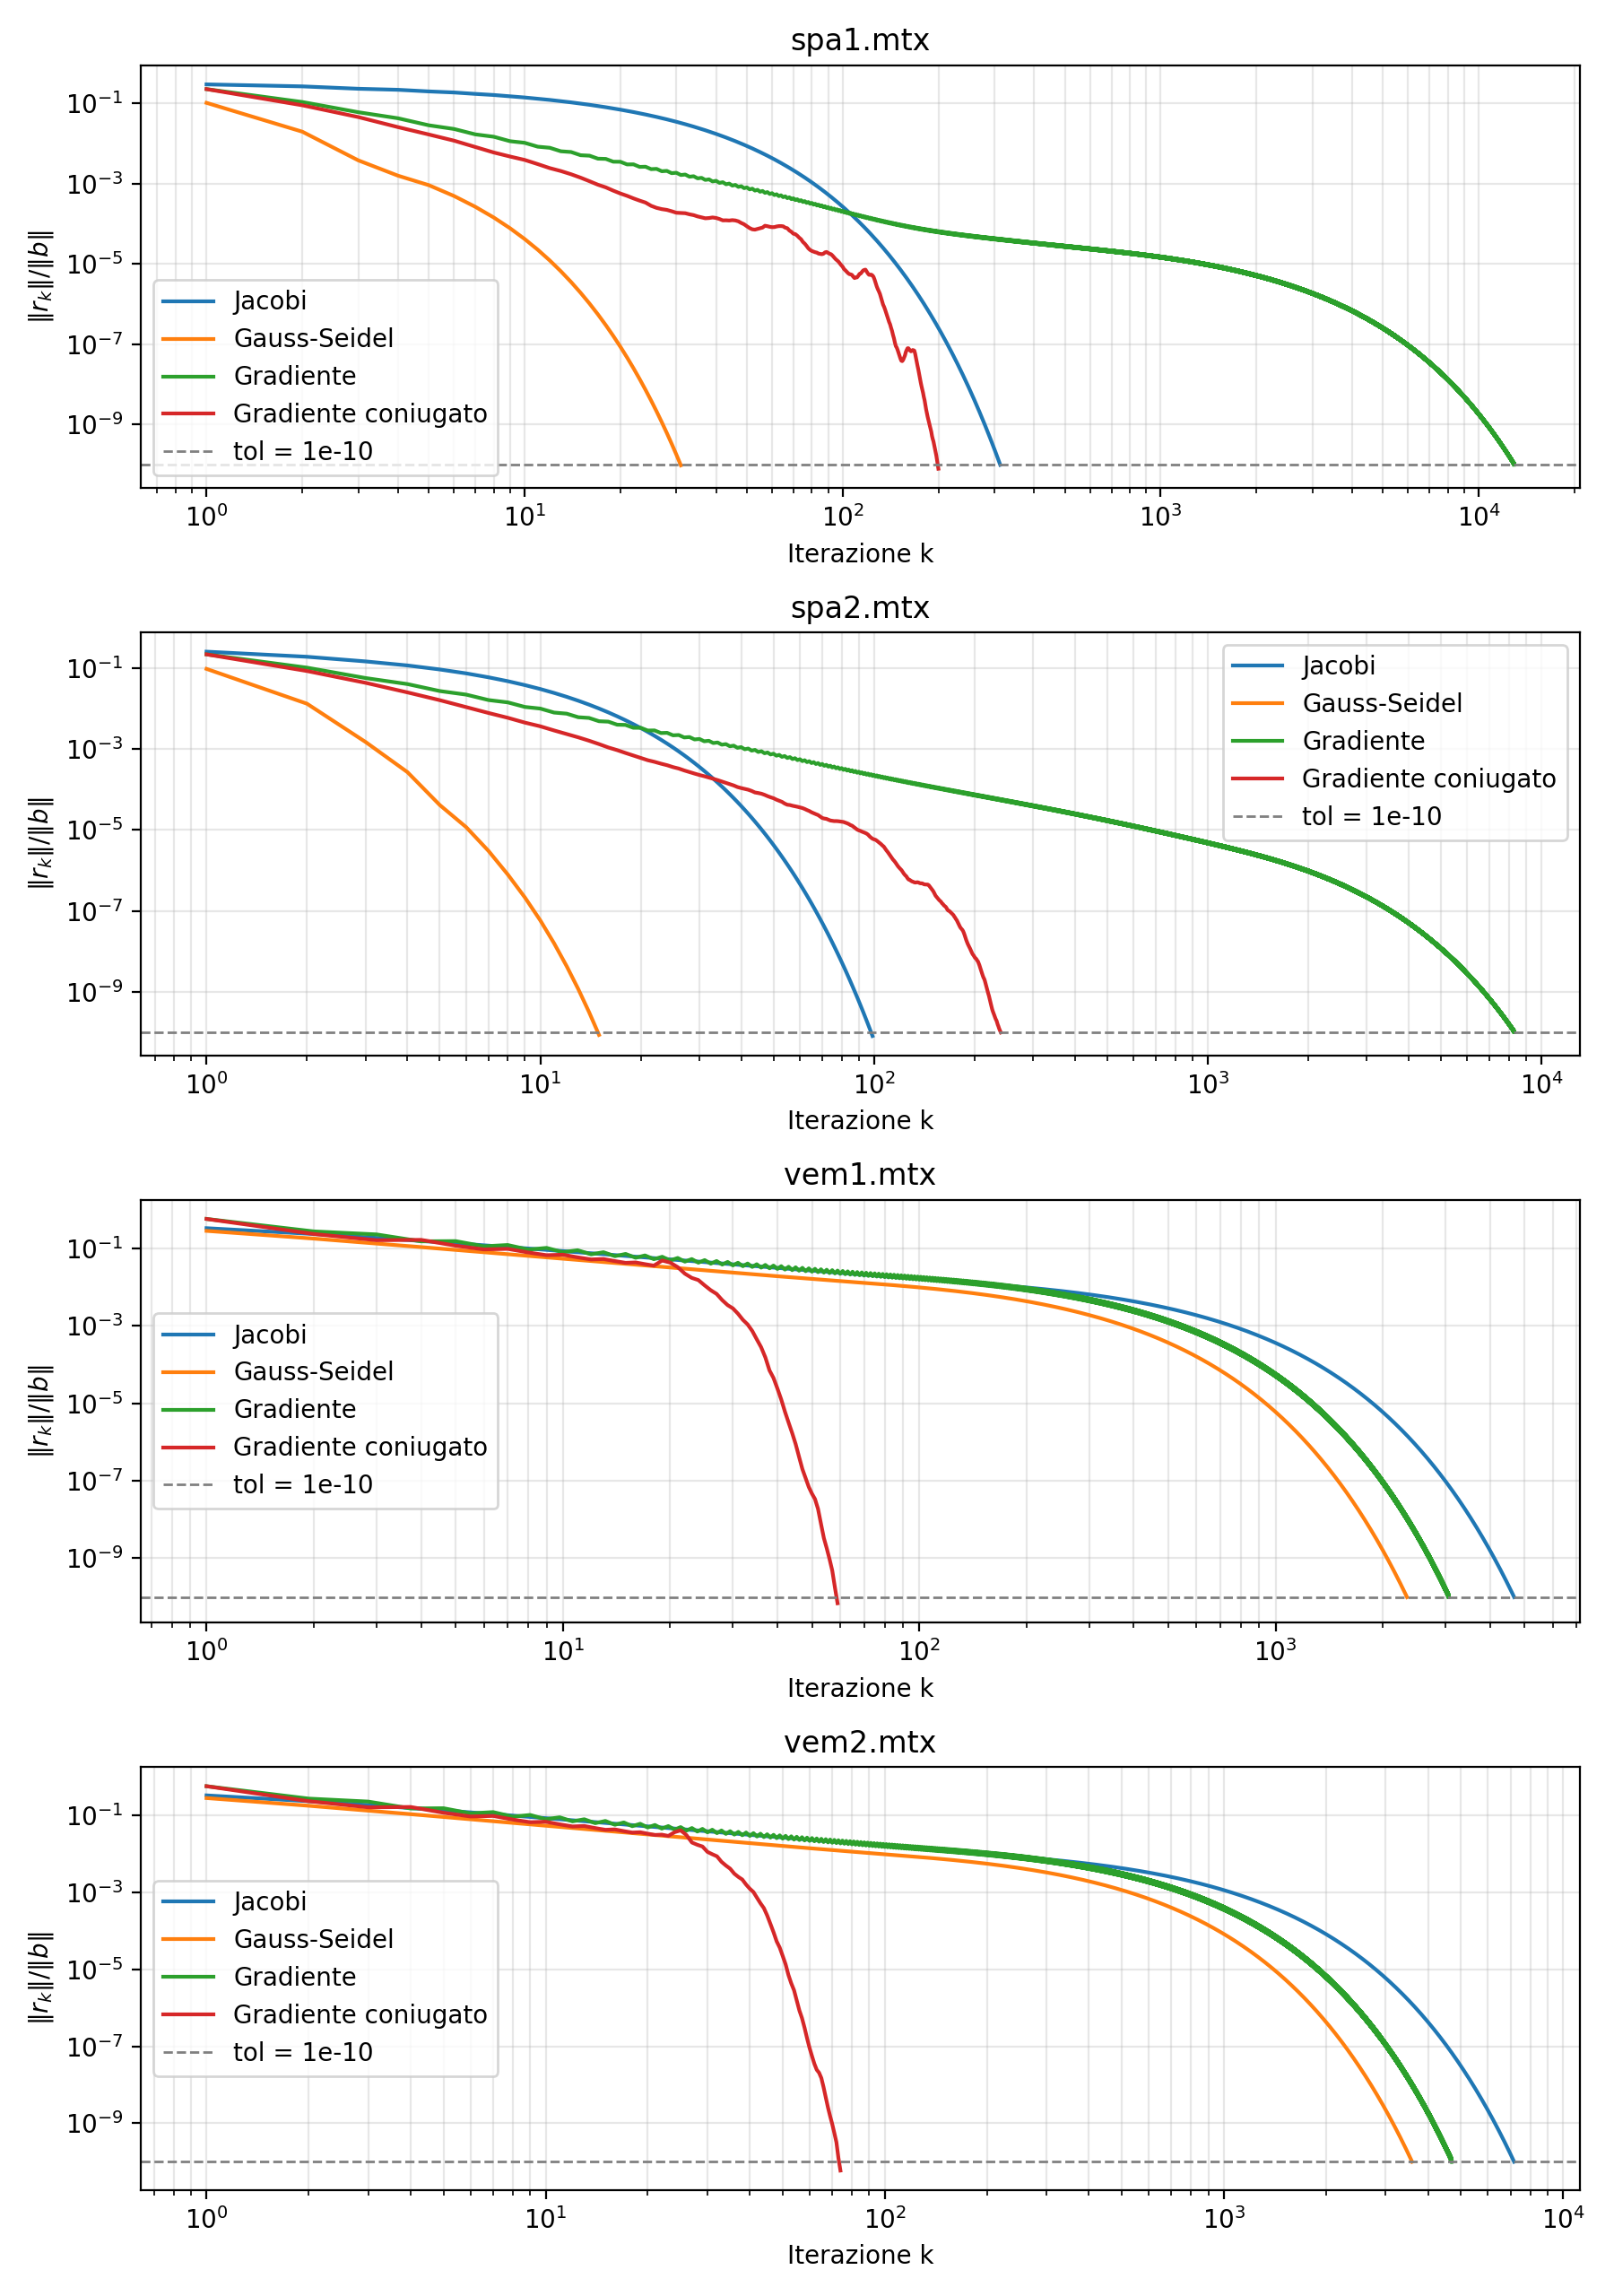
\includegraphics{../results/plots/convergence.png}}

\begin{frame}{Storia di convergenza 1}
    \begin{figure}
        \centering
        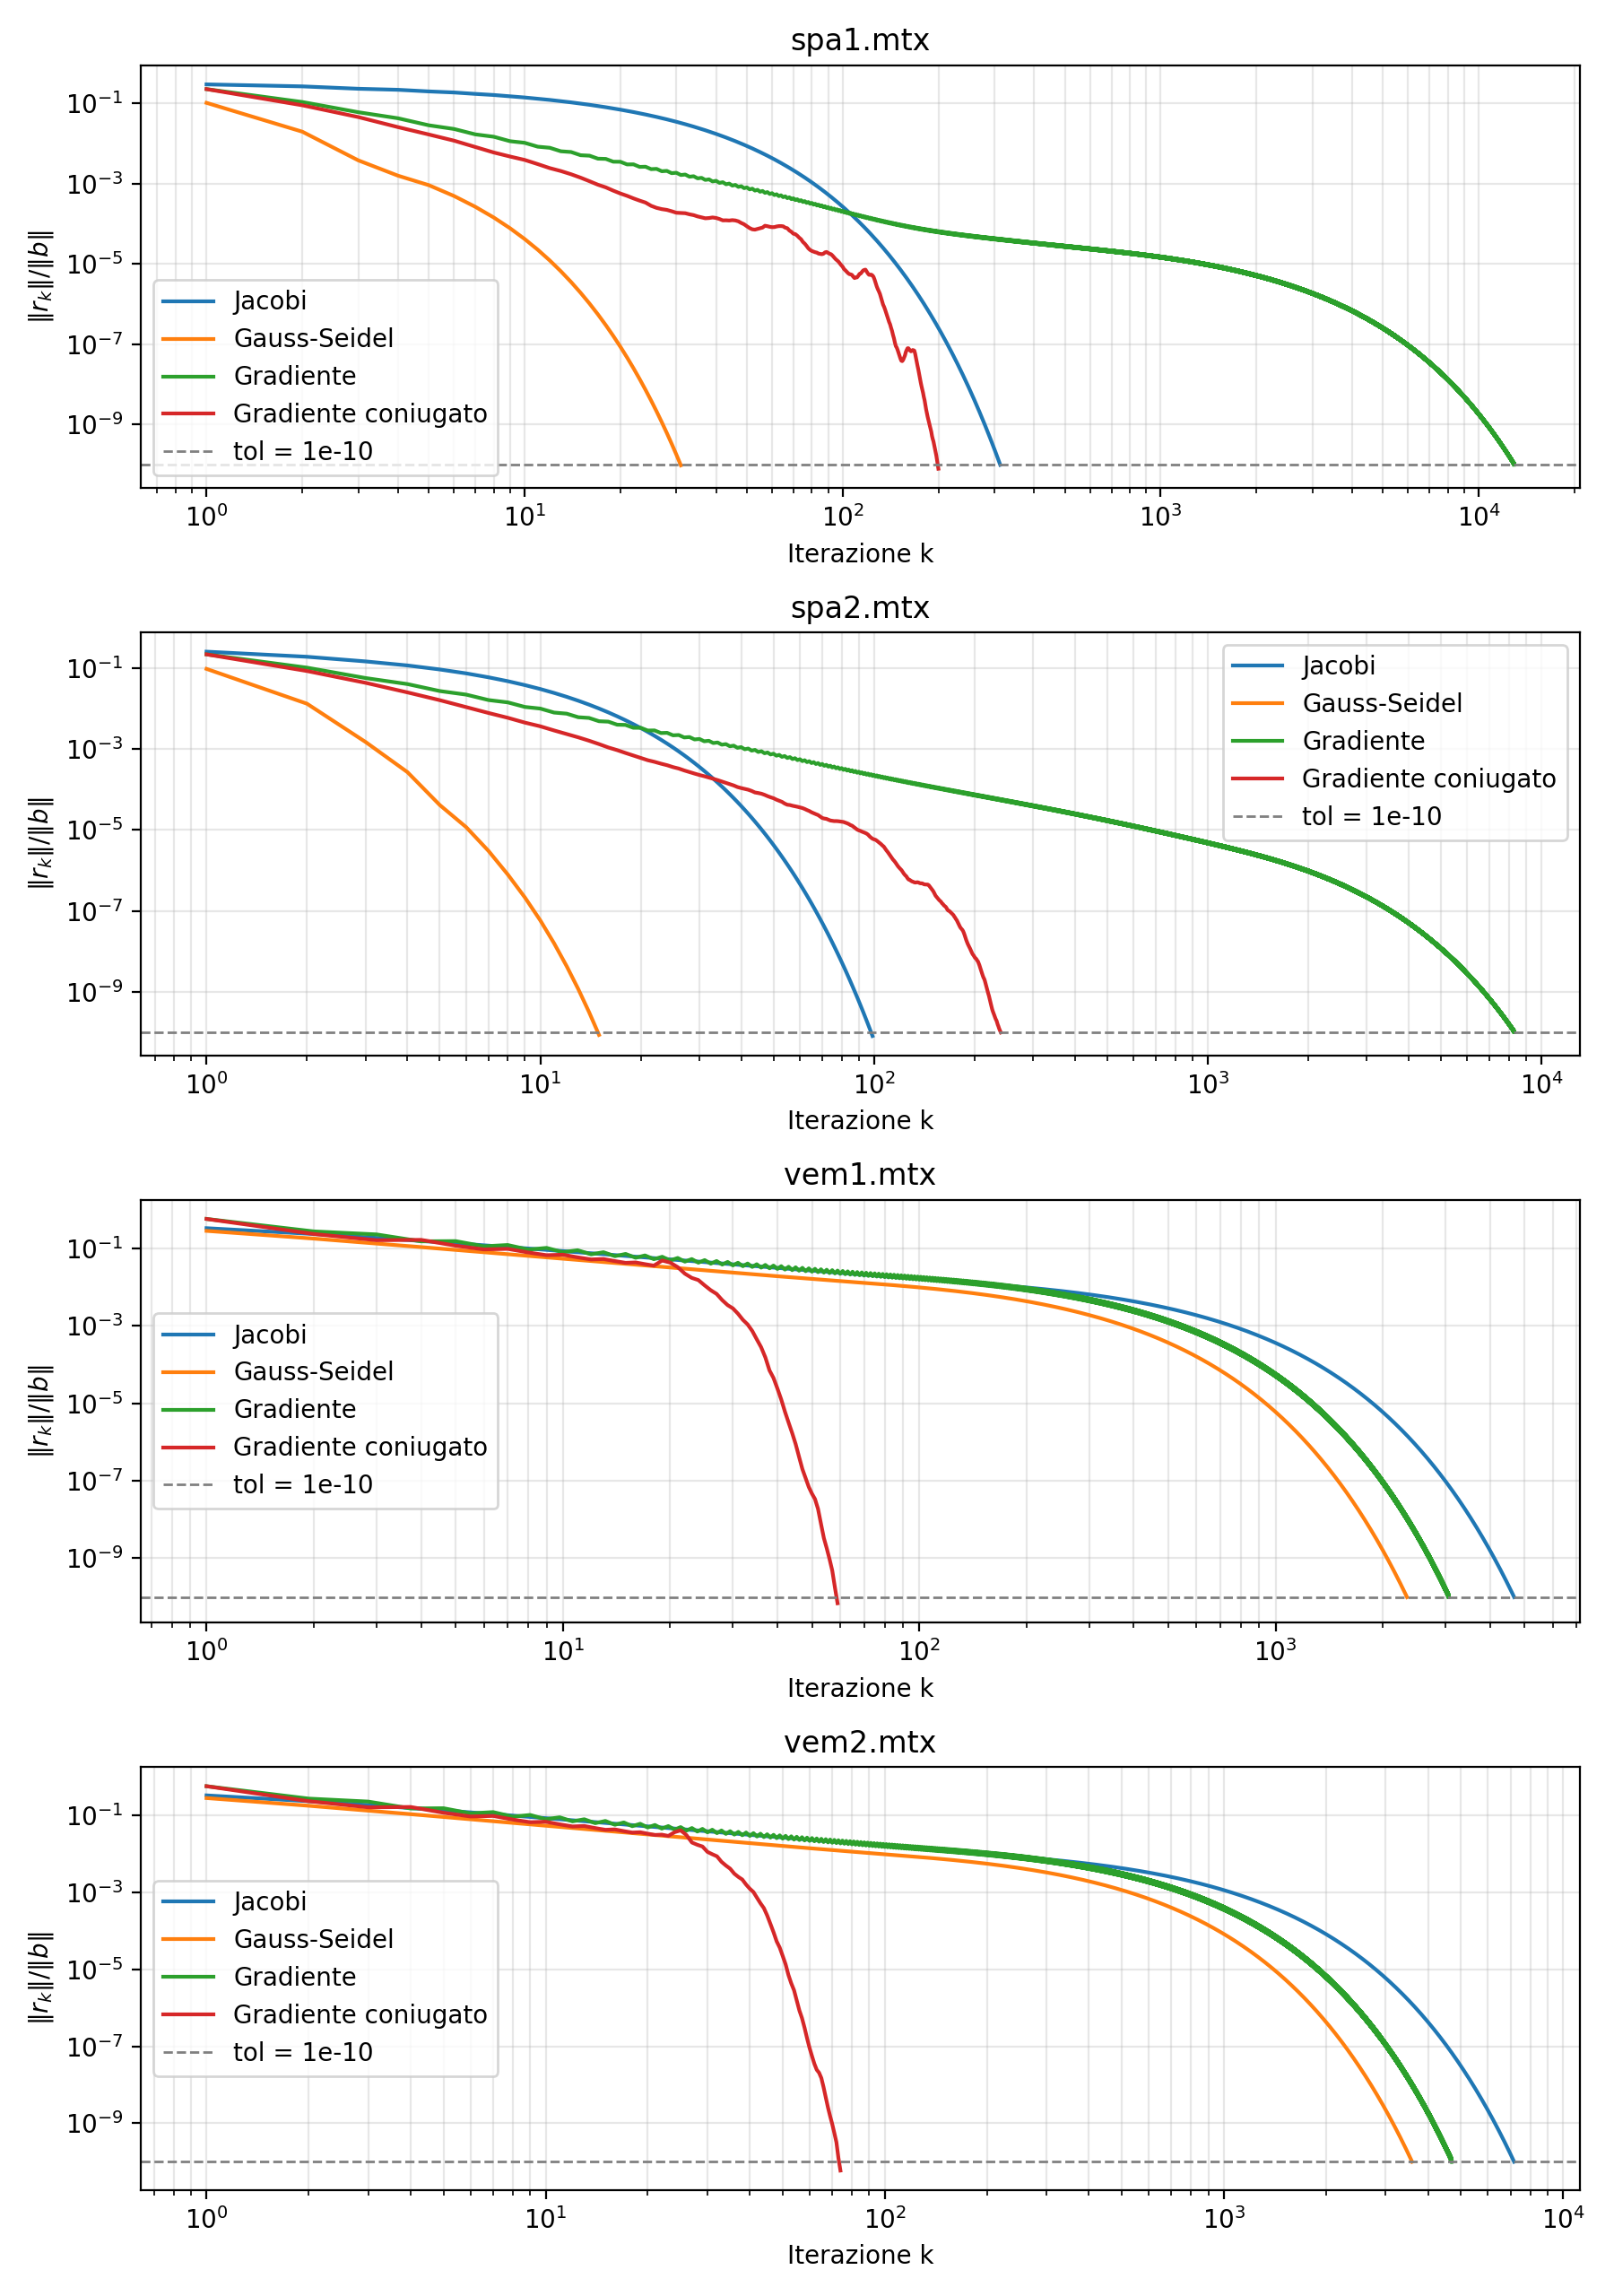
\includegraphics[trim=0pt {0.5\ht\convbox} 0pt 0pt, clip, width=\textwidth, height=0.85\textheight, keepaspectratio]{../results/plots/convergence.png}
    \end{figure}
\end{frame}

\begin{frame}{Storia di convergenza 2}
    \begin{figure}
        \centering
        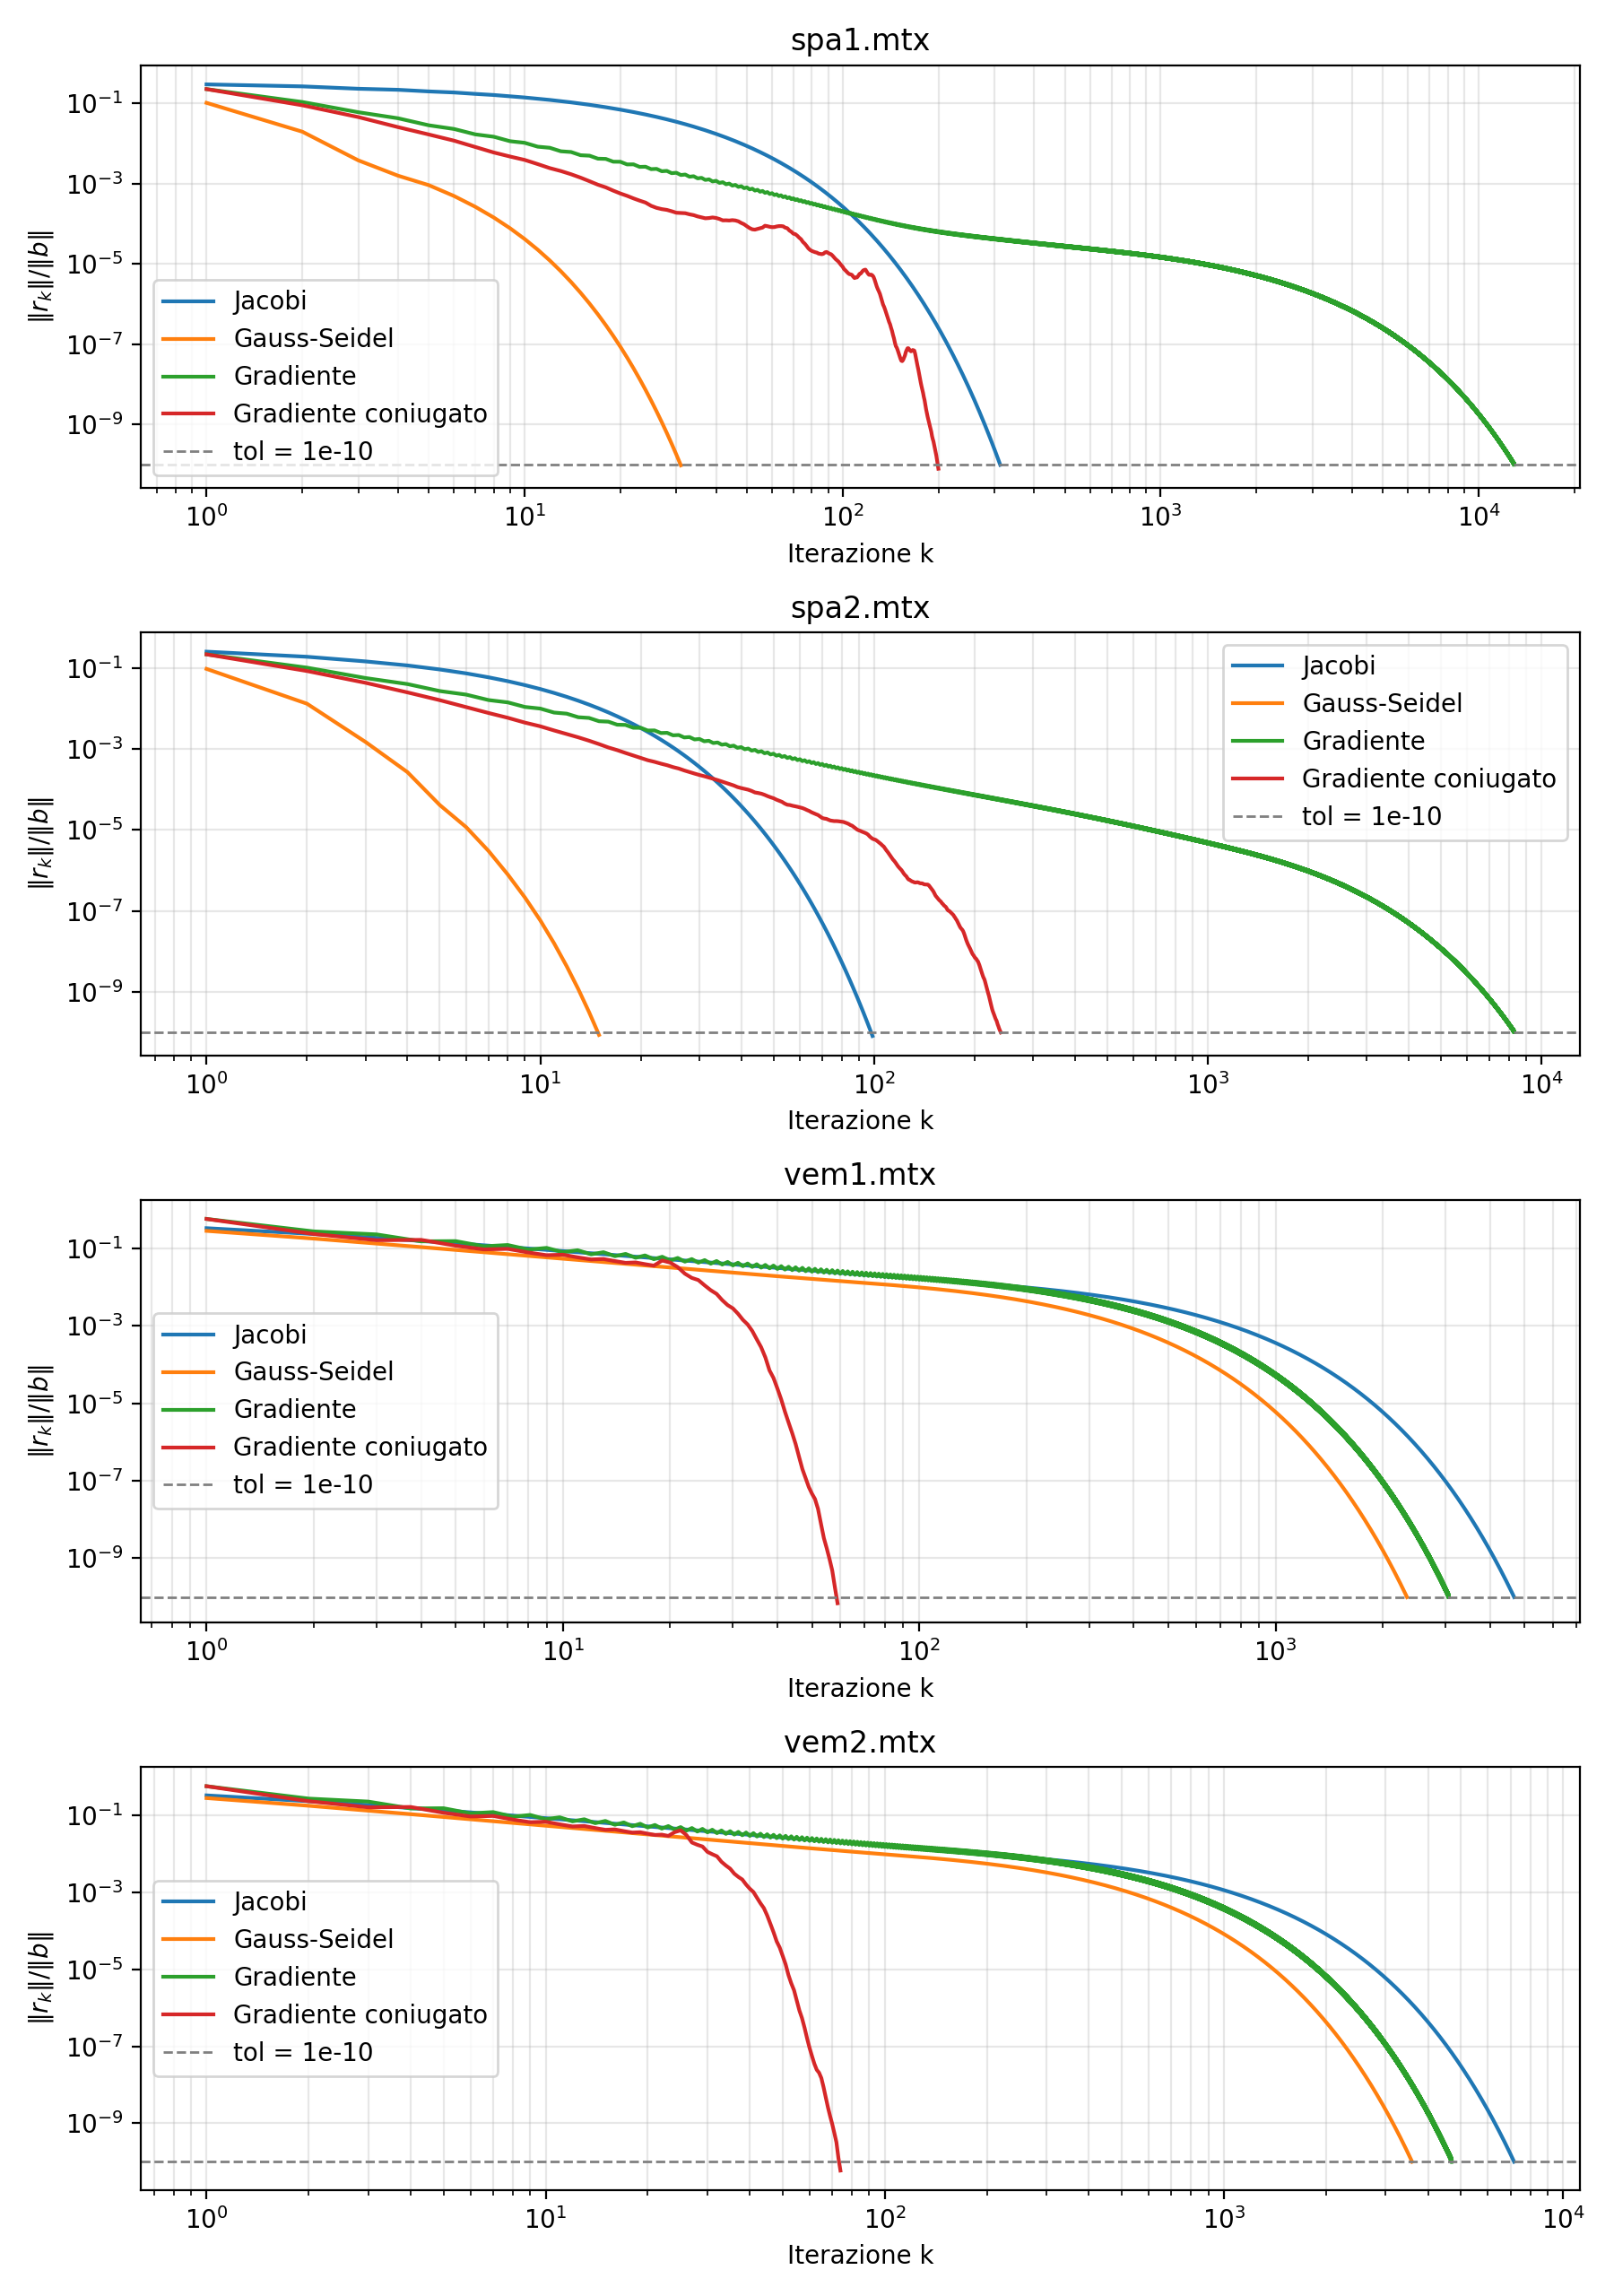
\includegraphics[trim=0pt 0pt 0pt {0.5\ht\convbox}, clip, width=\textwidth, height=0.85\textheight, keepaspectratio]{../results/plots/convergence.png}
    \end{figure}
\end{frame}

\begin{frame}{Condizionamento e Costo del singolo passaggio}
    \begin{itemize}
        \item I risultati pratici ottenuti nel test ricalcano perfettamente le crescite teoriche attese dalle equazioni.
        \item Il singolo passo di Gauss-Seidel porta a tempi fissi d'esecuzione maggiori a causa del blocco sequenziale.
    \end{itemize}
\end{frame}


\begin{frame}{Costo medio per operazione}
    \begin{figure}
        \centering
        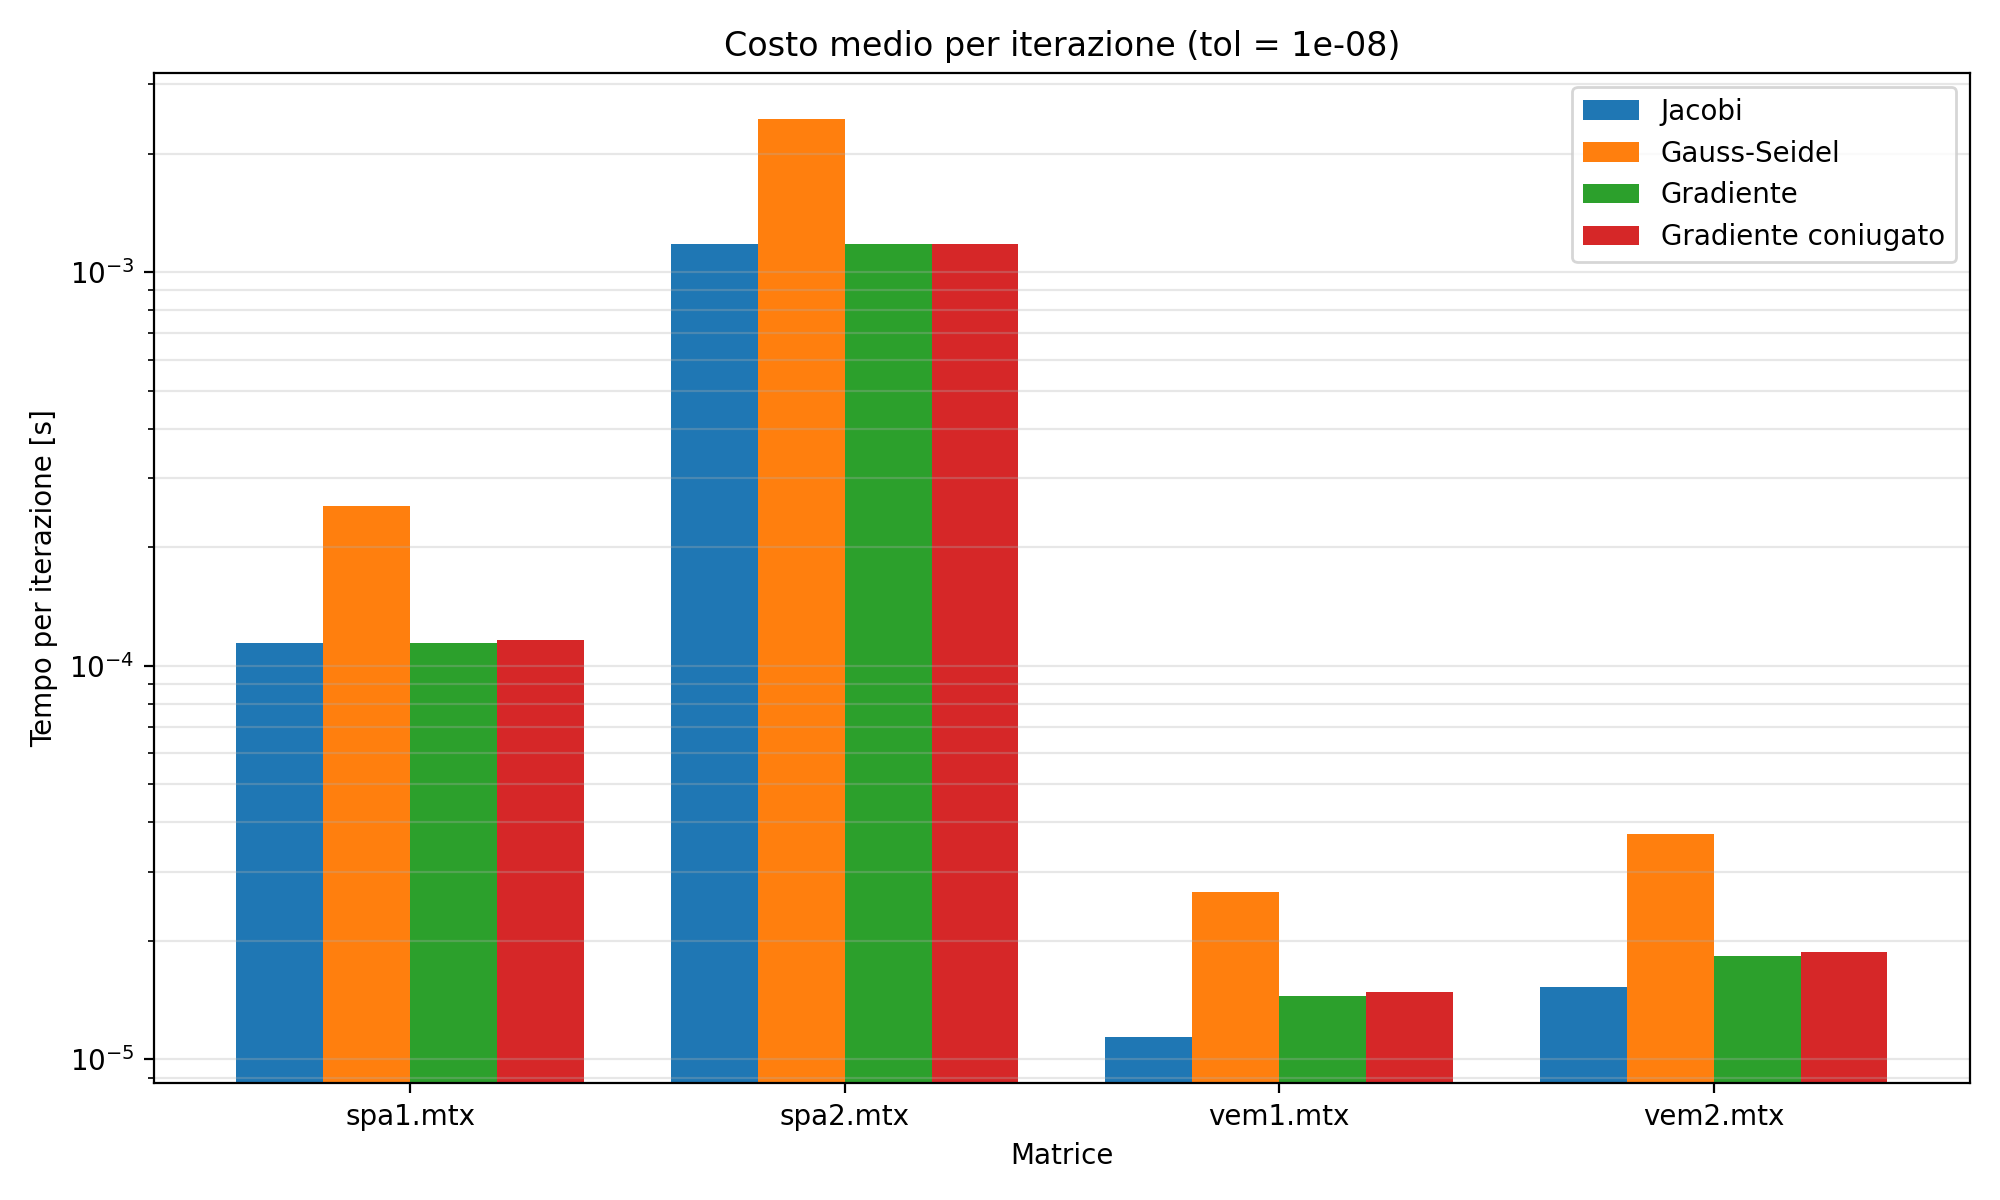
\includegraphics[width=\textwidth,height=0.85\textheight,keepaspectratio]{../results/plots/cost_per_iter.png}
    \end{figure}
\end{frame}

\begin{frame}{Riepilogo delle metriche essenziali}
    \begin{figure}
        \centering
        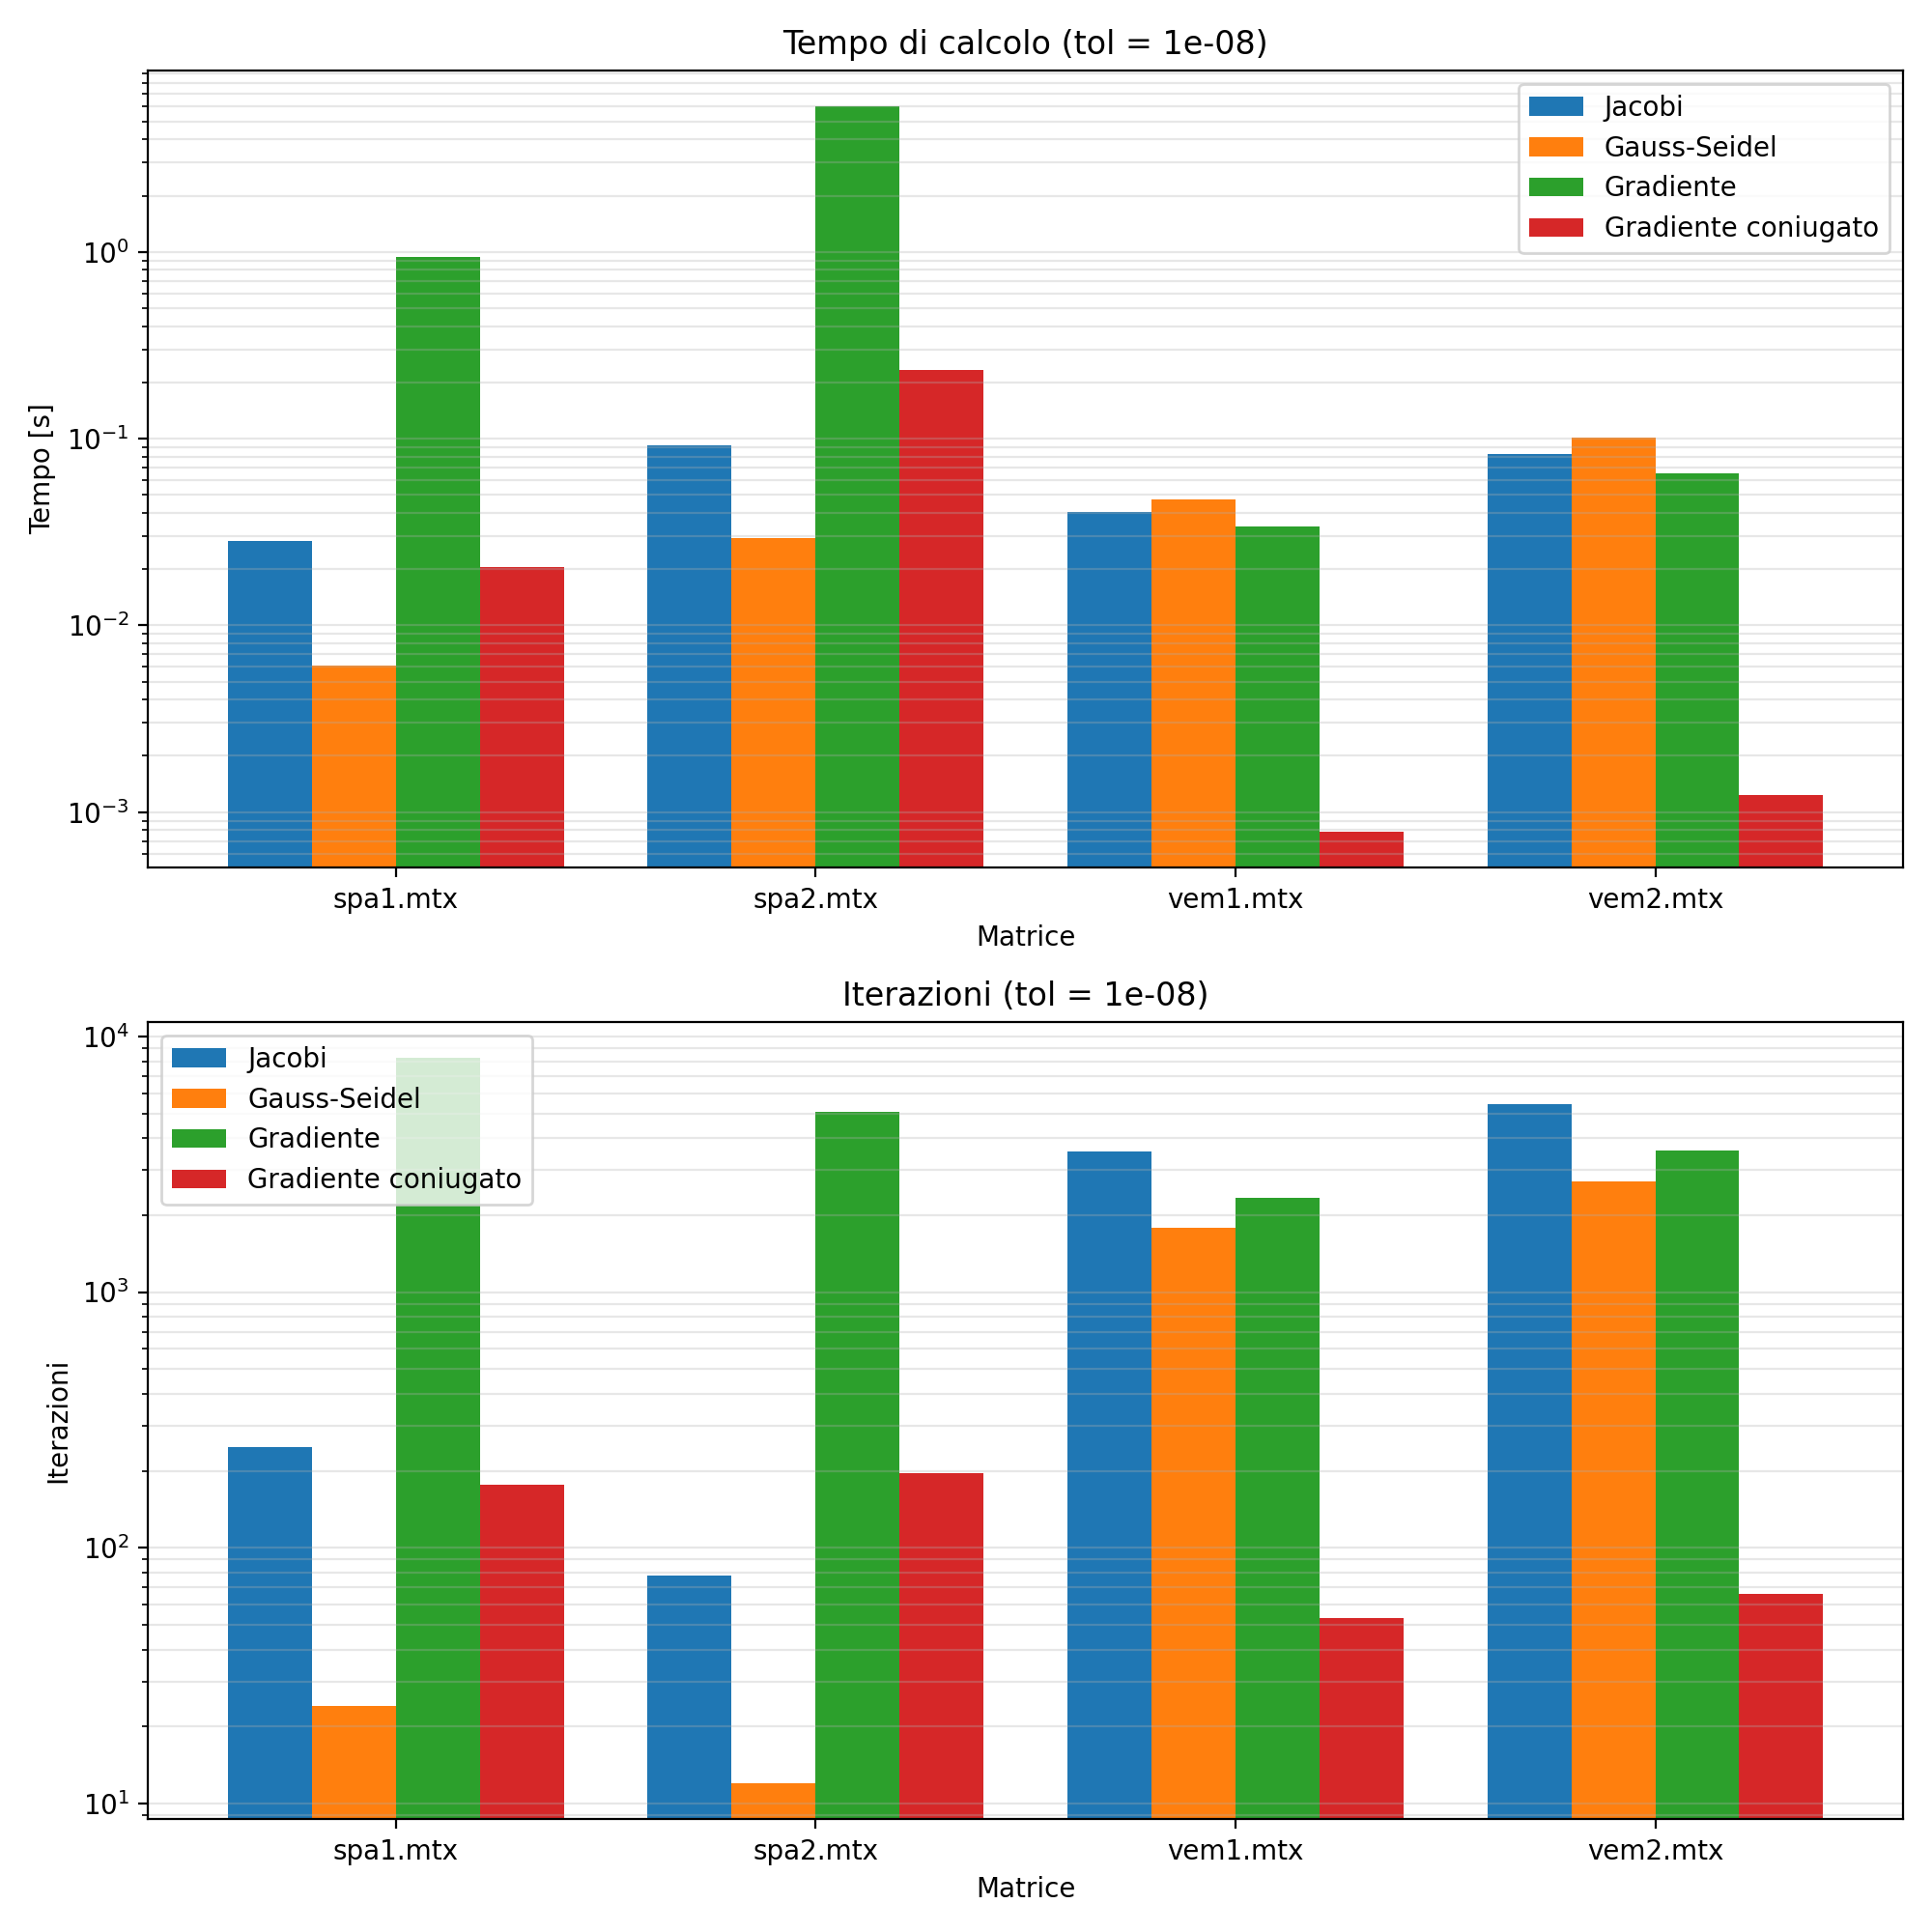
\includegraphics[width=\textwidth,height=0.85\textheight,keepaspectratio]{../results/plots/summary_bars.png}
    \end{figure}
\end{frame}

\section{Conclusioni}

\begin{frame}{Conclusioni}
    \begin{itemize}
        \item Il criterio di arresto basato sul residuo scalato si è dimostrato stabile ed efficace per ogni caso analizzato.
        \item Il gradiente coniugato è la scelta più robusta ed efficiente: annulla la discesa a zig-zag ed è il metodo più rapido per matrici molto sparse.
        \item Gauss-Seidel si difende in modo eccellente sulle matrici a media densità: il risparmio di iterazioni compensa il peso del singolo passo.
        \item Jacobi e gradiente semplice non risultano mai la scelta ottimale per le performance, ma restano essenziali come base matematica e di riferimento teorico.
    \end{itemize}
\end{frame}

\begin{frame}[plain]
    \begin{center}
        \Huge{Grazie per l'attenzione}
    \end{center}
\end{frame}

\end{document}
